\documentclass[12pt,a4paper,parskip]{scrartcl}
\usepackage[utf8]{inputenc}
\usepackage[T1]{fontenc}
\usepackage[ngerman]{babel}
\usepackage{lmodern}
\usepackage[babel,german=guillemets]{csquotes}
\usepackage[style=verbose-ibid,backend=bibtex8]{biblatex}
\bibliography{baclit100214}
\usepackage{amsmath}
\usepackage{amsfonts}
\usepackage{amssymb}
\usepackage{makeidx}
\usepackage{graphicx}
\usepackage{url}
\usepackage[locale=DE]{siunitx}%SI Einheiten etc.
\usepackage[german]{fancyref}%möglicherweise rausnehmen oder justieren
\usepackage{booktabs} %Tabellen Horizontale Linier dick darstellen
\usepackage{rotating}
\usepackage{lscape}
\usepackage{subfig}
\usepackage[left=3cm,right=3cm,top=2cm,bottom=2cm]{geometry}
\begin{document}
\author{Benedikt Kaffanke}
\title{Einfluss des Ausgangs- und  Werkzeugmaterials auf Umformprozesse zur Herstellung von Verzierungselementen in der Automobilbranche}
\maketitle
\newpage
\tableofcontents
\newpage
\section{Einleitung}
In der modernen Automobilindustrie werden heutzutage immer höhere Qualitäts- und Präzisionsansprüche an die einzelnen Fahrzeugkomponenten  gestellt. So unterliegen selbst Verzierungselemente strengen Maß- und Toleranzvorgaben von Seiten der Hersteller an die Komponenten Zulieferer.\\
 Die Fertigungsprozesse solcher Präzisionsfabrikate erfordern ein hohes Maß an Überwachung und Kontrolle auf den einzelnen Fertigungsstufen. Es kommen überwiegend modernste Fertigungstechnologien (CNC-Maschinen, Industrie Roboter) zum Einsatz. Trotz hohem Automatisierungsgrad sind immer noch humane Fertigungskräfte unverzichtbar. So ist zum Beispiel bei einer \emph{Sichtprüfung} zur Verifikation der erforderlichen Oberflächengüte, des bearbeiteten Materials,  das menschliche Auge unersetzlich. Auch das Handling bei Nacharbeitungsverfahren (z.B. Polieren, Schleifen) geschieht häufig noch manuell. So  erstreckt sich das Spektrum der am Fertigungsprozess Involvierten von der einfachen Hilfskraft bis zum hochqualifizierten CNC-Spezialisten.\\
  Hinter diesem Background ist es nicht zu vermeiden das eine komplexe Anzahl von Einflussgrößen bei der Wertschöpfung als Störfaktor berücksichtigt werden müssen. Eine besondere und stetige Observation, insbesondere bei der Herstellung von sehr großen Stückzahlen,  des kontinuierlichen Flusses der Bearbeitungsschritte und der Synergie der einzelnen Elemente  der Fertigungskette, ist daher ein wichtiger Punkt zur Prävention eventueller negativer Störfaktoren. Muss zum Beispiel eine Bearbeitungsstufe, während einer Serienfertigung an einer CNC-Einheit,  aufgrund von inhomogenen Spannungsverläufen im Ausgangsmaterial häufig unterbrochen werden um Justierungen an dem Gerät durch   qualifizierte Spezialisten vorzunehmen,  ist der Kosten- und Zeitaufwand wirtschaftlich nicht mehr vertretbar.\\
     Im Fokus dieser Forschungsarbeit steht deshalb die Problematik der Optimierung der Fertigungsverfahren zur Erlangung höherer Güte bei der Herstellung von Zierleisten.
 

Zum größten Teil werden für eben diese Verzierungselemente
Strangpressprofile aus Aluminium verwendet die ein besonders hochwertiges Finish verbürgen. Sie werden in speziellen Biege- und Abkantvorrichtungen in Serie gefertigt.
 Weitere Bearbeitungsprozesse sind: \begin{itemize}
 \item Fräsen
 \item Beschneiden
 \item Schleifen und Polieren
 \item Eloxieren
 \item DURAPro Beschichten (Nanolack)
 \item Montage
 \end{itemize}
   Besondere Schwierigkeiten treten im Bereich der Maßtoleranz Einhaltung bei diesen Biegeprozessen auf. Häufig sind bei  Biegeradien und langen Profilen Toleranzen von $\pm \SI{0.5}{\milli\meter}$ gefordert. Bei kleinen Biegeradien die größtenteils bei Abkantprozessen anfallen treten optische Merkmale und Veränderungen auf, die meistens unerwünscht sind.\\
 Die Beschaffenheit des Werkstoff- und Werkzeugmaterials ist der wohl wichtigste Beeinflussungsfaktor bei o.g. Problemprodukten (siehe \fref{fig:Verdeckkastendeckel}) .
 \begin{figure}[!htb]
 \centering
 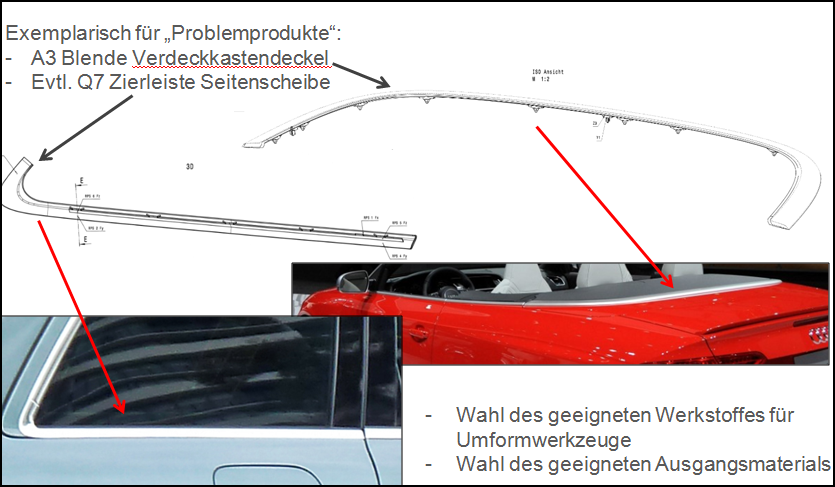
\includegraphics[scale=.54]{ZierleisteVerdeckklappendeckel}
 \caption{Problemprodukte Zierleisten und Verdeckkastendeckel}
 \label{fig:Verdeckkastendeckel}
 \end{figure}

Die nächsten Abschnitte befassen sich mit der Durchführung und Auswertung von Versuchsreihen die mit Hilfe von Messungen, herkömmlicher sowie zukunftsweisender Art (FEM-Verfahren), Erkenntnisse liefern  die die Herstellungsverfahren von Zierleisten  in qualitativer- sowie ökonomischer Sicht  optimieren.\\
Zur Untersuchung   sind hier vor allen Dingen die Umformverfahren  Kröpfen (siehe \fref{sec:kropf})  und Streckbiegen herangezogen worden. 


\newpage
\section{Exkurs Umformtechnik}


Da die Gegenstände und Verfahren dieser Untersuchung in das Gebiet der Umformtechnik fallen, werden die ausschlaggebendsten Begriffe und Sachverhalte dieses komplexen Gebietes noch einmal vereinfacht und komprimiert umrissen. So ist es möglich über ein theoretisches Gerüst zu verfügen welches später behilflich sein wird   Analogien zu den durchzuführenden Prozessen zu erkennen.
\subsection{Systematisierung Formgebungsverfahren}
Umformverfahren können
auf Grund der unterschiedlichen Spannungsverhältnisse in fünf verschiedene Gruppen unterteilt werden. Einfache Beschreibungen der Spannungsverhältnisse sind kaum möglich denn,  abhängig von der Art der Operation, können  unterschiedliche Spannungen gleichzeitig auftreten oder sich sogar  während des Formgebungsvorgangs verändern. Deshalb werden die überwiegenden Spannungen als Klassifikationskriterium ausgewählt. Folgende fünf Gruppen der Umformprozesse werden definiert:
\begin{enumerate}
\item \emph{Druckumformen} nach DIN 8583 behandelt die Formgebung eines festen Körpers  welche den  plastifizierten  Zustand hauptsächlich durch uni- oder multiaxiale Druckbelastungen herbeiführt.
\item \emph{Zugdruckumformen} nach DIN 8584 behandelt die Formgebung eines festen Körpers  welche den plastifizierten Zustand  hauptsächlich durch kombinierte uni- oder multiaxiale Zug- und Druckbelastungen herbeiführt.
\item \emph{Zugumformen} nach DIN 8585 behandelt die Formgebung eines festen Körpers welche den plastifizierten Zustand überwiegend durch uni- oder multiaxiale Zugbelastungen verursacht.
\item \emph{Biegeumformen} nach DIN 8586 behandelt die Formgebung eines festen Körpers welche den plastifizierten Zustand hauptsächlich durch eine Biegebelastung herbeiführt.
\item \emph{Schubumformen} nach DIN 8587 behandelt die Formgebung eines festen Körpers welche den plastifizierten Zustand überwiegend durch eine Schubbelastung herbeiführt.

\end{enumerate}

Von untergeordneter Bedeutung sind innerhalb dieser Gruppen  weitere Unterteilungen auf der Grundlage von kinematischen Überlegungen (z.B. Relativbewegung zwischen Werkzeug und Werkstück), Werkzeug- und Werkstück Geometrien sowie Beziehungen zwischen den beiden möglich. Die Klassifizierung formgebender Methoden unterlässt bewusst die Frage ob ein Prozess durch Erwärmung, bei Raumtemperatur oder weiterer Wärmebehandlung stattfindet. Früher  wurde zur Abgrenzung zwischen Kalt- und Warmformen die Rekristallisationstemperatur gewählt. Obwohl diese sicherlich das Verhalten  von Werkstückmaterialien während der Formgebung beeinflusst, zählt heutzutage zur Allgemeinerkenntnis das die spontane Erholung  eine weitaus größere Rolle in schnellen Umformprozessen spielt. Außerdem führt die herkömmliche Terminologie angesichts der großen Vielfalt  an Materialien die verwendet werden leicht zu Missverständnissen. So würde zum Beispiel die Formgebung von Blei bei Raumtemperatur als \emph{Warmumformen} deklariert während Molybdän bei einer Temperatur von 800 Grad Celsius noch als \emph{Kaltumformen} eingestuft wäre. Aus diesem Grunde unterscheidet DIN 8582 zwischen Formgebung bei Raumtemperatur und Formgebung bei einem auf über Raumtemperatur erwärmten Werkstücks. Überdies ist zu Berücksichtigen ob ein permanenter Temperaturwechsel während des Umformvorgangs stattfindet. Mit Hilfe dieser beiden Kriterien ist eine weiter Unterteilung von den Metall Umformverfahren möglich:

\begin{enumerate}
\item Formgebung nach Erwärmung (Warmumformen)
\item Formgebung ohne Erwärmung (Kaltumformen)
\end{enumerate}

Beide Punkte können weiter eingestuft werden in:

\begin{itemize}
\item Formgebung ohne Veränderung der mechanischen Eigenschaften
\item Formgebung mit temporärer Veränderung der mechanischen Eigenschaften
\item Formgebung mit permanenter Veränderung der mechanischen Eigenschaften
\end{itemize}

In der Industriepraxis kommen letztendlich unzählige Kombinationen der oben aufgeführten Unterteilungen vor.\footcite[Vgl.][2.1ff]{kl}
\subsection{Metallurgische Zusammenhänge}
In diesem Abschnitt wird erörtert was auf makroskopischer und mikroskopischer Ebene in metallischen Werkstoffen bei Formänderungsprozessen vor sich geht. Überdies soll ein Einblick gewonnen werden wie sich die verschiedenen Einflussgrößen während eines Umformvorgangs gegenseitig beeinflussen.
\subsubsection{Kristallaufbau}
In der Umformtechnik werden zum Großteil metallische Bauteile erzeugt. Eisen- wie Nichteisenmetalle bestehen aus metallisch gebundenen Atomen. Sie bekommen ihren Zusammenhalt aus einer sie gleichmäßig umgebenden frei beweglichen Elektronengaswolke, die aus abgegebenen Valenzelektronen besteht und so die positiven Metallionen  durch die sogenannte \emph{Metallbindung} bindet.\footcite[Vgl.][12]{wki} Ihr wichtigstes Merkmal ist der kristalline Aufbau. Darunter versteht man die feste, regelmäßige Struktur der Atome. In der Physik sowie in der Chemie existieren verschiedene Modelle über den Aufbau und das Aussehen solcher Kristallgebilde. In \fref{fig:makromikro}\footcite[Vgl.][4]{fu} wird eine Elementarzelle des $\alpha $-Eisen unter mikroskopischen (atomistischen) und makroskopischen Gesichtspunkten dargestellt. Oben rechts im Bild sind die drei Elementarzellen abgebildet aus denen Metalle zusammengesetzt sind. Es handelt sich um die  kubisch-raumzentrierte , kubisch-flächenzentrierte und hexagonale (das hdP steht für hexagonal dichteste Packung) Elementarzellen.\footcite[Vgl.][3-5]{fu}
\begin{figure}[hbtp]
\centering
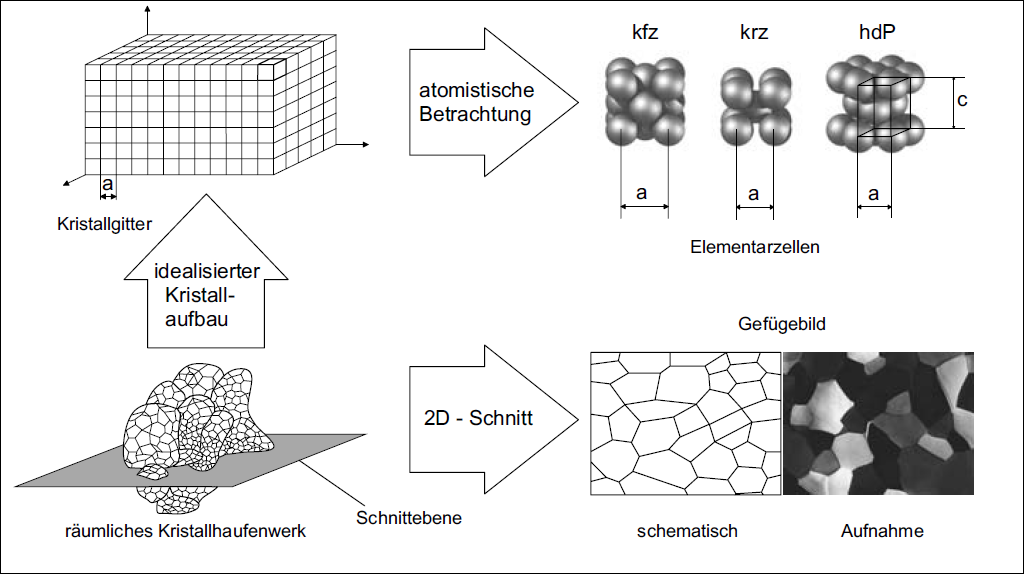
\includegraphics[scale=.54]{makromikro}
\caption{Aufbau eines Kristallgitter mikroskopisch (atomistisch) und makroskopisch.}
\label{fig:makromikro}
\end{figure}
Das kleinste Kristall im Metallgitterverband ist das sogenannte \emph{Einkristall} (siehe \fref{fig:elementarzellen})\footcite[Vgl.][37]{hu} es besitzt folgende Merkmale\begin{itemize}
\item allseitig freie Oberfläche
\item keine Korngrenzen
\item Fehlstellen wie z.B. Leerstellen, Versetzungen
\item anisotropisches Verhalten wegen bevorzugter Gleitrichtungen. Unter \emph{Anisotropie} wird das Auftreten von unterschiedlichen mechanischen und physikalischen Eigenschaften in die verschiedenen Raumrichtungen verstanden (z.B. Sperrholz). Im Gegensatz dazu weist \emph{isotropisches} Verhalten gleiche mechanische und physikalische Eigenschaften in die verschiedenen Raumrichtungen auf (z.B. Sonnenlicht)\footcite[vgl.][37]{hu}
\begin{figure}[hbtp]
\caption{Elementarzellen (Einkristalle)}
\centering
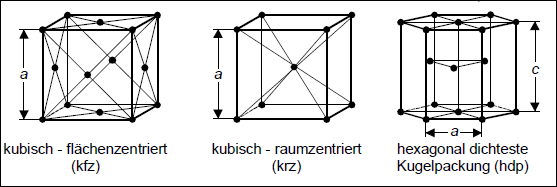
\includegraphics[scale=1]{elementarzellen}
\label{fig:elementarzellen}
\end{figure}

\end{itemize}
Die kleinste geometrisch zusammenhängende Einheit eines Kristallgitters ist die Elementarzelle. Knüpft man hypothetisch, in Richtung aller drei Koordinatenrichtungen, Elementarzellen aneinander entsteht ein Kristallgitter (siehe \fref{fig:makromikro} oben links). Das geometrische Aneinanderreihen von Elementarzellen erzeugt \emph{Idealkristalle} (fehlerfreie Kristalle) die so in der Realität nicht vorhanden sind. In der Realität sind in einem Raumgitter der Metalle zahlreiche Gitterfehler vorhanden. Hier wird unterschieden in folgende signifikante Gitterfehler:
\begin{enumerate}
\item  \emph{Nulldimensionale Gitterfehler} (punktförmig):\begin{itemize}
\item \emph{Zwischengitteratome} liegen vor wenn Atome auf Zwischengitterplätzen angeordnet sind. 
\item \emph{Austausch- oder Substitutionsatome}. Die Atomplätze werden von Fremdatomen beansprucht.
\item \emph{Einlagerungsatome} entstehen wenn die Zwischengitterplätze von Fremdatomen vereinnahmt werden.
\item \emph{Leerstellen} treten auf wenn wenn einzelne Gitterplätze nicht von Atomen besetzt werden. Sie sind bedeutend bei thermisch aktivierten Diffusionsvorgängen.
\end{itemize}
\item \emph{Eindimensionale Gitterfehler} sind linienförmige Strukturfehler (Versetzungen)(siehe \fref{fig:versetzung})\footcite[Vgl.][50]{wk}.

\begin{figure}[hbtp]
\centering
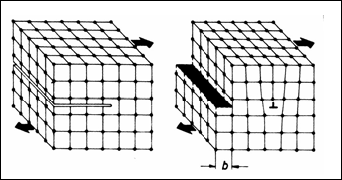
\includegraphics[scale=1.53]{versetzung}
\caption{Stufenversetzung}
\label{fig:versetzung}
\end{figure}
 Diese sind für Umformprozesse von übergeordneter Bedeutung weil sie die plastische Formgebung besonders beeinflussen.
\item \emph{Zweidimensionale Gitterfehler} entstehen bei Oberflächendefekten. Die wichtigsten sind Korngrenzen und Phasengrenzflächen. Wenn ein Metall aus dem flüssigen Zustand kristallisiert wachsen die Keime zuerst an verschiedenen Stellen unabhängig voneinander. Im Laufe des Abkühlungsprozesses wachsen die Keim aufeinander zu und bilden Korngrenzen.
\end{enumerate}

Der Unterschied zwischen Real- und Idealkristallen ist in diesen Gitterfehlern begründet. Die Zugfestigkeit des Eisens liegt  z.B mehr als zwei Zehnerpotenzen unter der theoretisch Möglichen im Fall des Vorhandenseins eines Idealkristalls. Die Abstände der Atome sind in den Elementarzellen in verschiedene Richtungen unterschiedlich ausgeprägt. Das ist die Ursache für die Richtungsabhängigkeit bestimmter Eigenschaften der Metalle. Bestimmte Herstellungsverfahren (z.B. einige Walzverfahren, gerichtete Erstarrung) zielen darauf ab die Orientierung der Kristallite in eine bestimmte Richtung zu beeinflussen. Dieses Vorgehen bezeichnet man als Textur. Sie ermöglicht das die Werkstoffeigenschaften richtungsabhängig werden.  Die Richtungsabhängigkeit wird wie schon oben erwähnt mit dem Begriff der \emph{Anisotropie}. 
Während des Erstarrungsprozesses technischer Schmelzen werden Verunreinigungen überwiegend vor der Erstarrungsfront hergeschoben. Es bilden sich Ansammlungen von Verunreinigungen an den Korngrenzen. Ein reales Gefüge ist durch einen metallogfrafischen Schliff im Lichtmikroskop zu erkennen und mit einem schematischem Gefüge verglichen (siehe \fref{fig:makromikro}) . Es sind lediglich Größe, Anordnung und Form der Kristalle erkennbar zu machen. Die innere Struktur ist nicht sichtbar zu machen.\footcite[Vgl.][3-6]{fu}

\subsubsection{Verformung Prinzipiell}
Die Duktilität (plastische Verformbarkeit) der Metalle ist eine Eigenschaft welche in der Umformtechnik die größte Bedeutung hat. Hier ist es sinnvoll die Vorgänge wieder an einem Idealkristall (besitzt keine Gitterfehler) darzustellen. Bei geringen Belastungen tritt im Bauteil keine bleibende Verformung ein, es geht nach  der Entlastung wieder in seinen Ausgangzustand zurück. Man nennt dies \emph{elastische} Verformung. Bei der \emph{plastischen} Verformung gleiten Kugelschichten im Gitterverband aneinander vorbei,  nach Entlastung kehrt das Bauteil nicht mehr in seine ursprüngliche geometrische Form zurück (siehe \fref{fig:eloplastkristall})\footcite[Vgl.][45]{wk}.
\begin{figure}[hbtp]
\centering
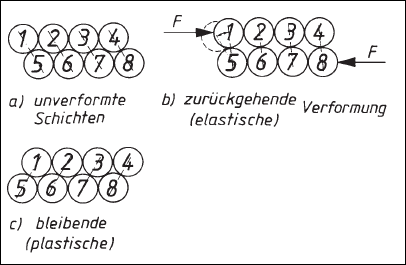
\includegraphics[scale=1.3]{eloplastkristall}
\caption{Verformung elastisch und plastisch}
\label{fig:eloplastkristall} 
\end{figure}
Das die plastische Verformung begünstigende Gleiten findet in den sogenannten \emph{Gleitebenen} statt. Diese befinden sich zwischen den Atomschichten mit der größten \emph{Packungsdichte}. Aufgrund dieser höheren Packungsdichte ist der Abstand der einzelnen Schichten nicht so groß und dem Verschieben der Schicht wird dort der  geringste Widerstand entgegengesetzt. Im Gegensatz zum Idealkristall sind aufgrund von Versetzungen die kritischen Schubspannungen, welche zur plastischen Verformung benötigt werden,  erheblich kleiner. Bei dem Idealkristall stellen wir uns ein schrittweises Gleiten ganzer Atomschichten vor während bei Realkristallen ein schrittweises Wandern der Atomreihen entlang der Versetzungslinien stattfindet. Man kann dies auch mit dem Wandern einer Teppichfalte vergleichen (siehe \fref{fig:wandernstufenversetzung}) \footcite[Vgl.][53]{wk}. Wenn z.B. ein sehr langer schwerer Teppich eine Falte hat erfordert es hohe Kräfte um durch Zug an einem Teppichende die Falte zu glätten. Wesentlich geringer ist der Kraftaufwand wenn man die Falte direkt langsam aus dem Teppich kämmt.\footcite[Vgl.][45-53]{wk}
\begin{figure}[hbtp]
\centering
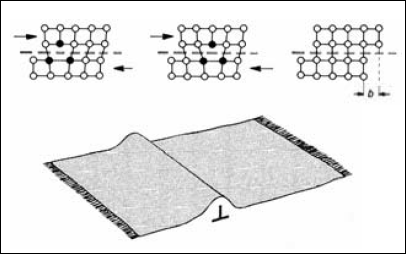
\includegraphics[scale=1.3]{wandernstufenversetzung}
\caption{Wandern einer Stufenversetzung in Analogie zum Wandern einer Teppichfalte}
\label{fig:wandernstufenversetzung}
\end{figure}




\subsection{Eigenspannungen}
Das Thema Eigenspannungen im Zusammenhang mit der Verarbeitung von Blechen an die hohe Qualitätsanforderungen gestellt werden ist natürlich von besonderem Interesse bei der Analyse von Problemstellungen die auf den einzelnen Fertigungsstufen entstehen können. Es handelt sich dabei um Spannungen in einem sich im Temperaturgleichgewicht befindenden Bauteil, auf das keine mechanischen Beanspruchungen wirken. Die mit den Eigenspannungen involvierten  Beanspruchungen stehen im mechanischen Gleichgewicht zueinander. Bei Bauteilen und Werkstücken die unter Eigenspannung stehen kann ein Materialversagen wesentlich schneller eintreten da sich die tatsächlich wirkende Spannung aus Eigenspannungen und Spannungen von außen einwirkenden Kräften zusammensetzt. Durch die Eigenspannungen kann auf Grund des daraus resultierenden gestörten Gleichgewichtszustands plastische Formänderung in Form von Verzug auftreten.
Dabei wirken sich Druckeigenspannungen in der Bauteilrandzone meist vorteilhaft aus da sie einer möglichen Rissbildung und Rissausbreitung entgegenwirken.

Es wird im Hinblick auf Auswirkungen auf das Bauteilvolumen eine Unterteilung der Eigenspannungen in drei Gruppen unternommen:
\begin{enumerate}
\item \emph{Makroskopische Eigenspannungen}, welche sich homogen über mehrere Kristallite erstrecken. Bei Störung des Gleichgewichts führen sie zu makroskopischen Formänderungen.
\item \emph{Eigenspannungen}, die in kleinen Abschnitten homogen sind und bei Störungen des Gleichgewichts zu makroskopischen Formänderungen führen.
\item \emph{Mikroskopische Eigenspannungen}, welche durch inhomogene Versetzungsreihen ausgelöst werden und über wenige Atombereiche variieren. Sie tragen nicht zu makroskopischen Formänderungen bei. 


\end{enumerate}

Eigenspannungen werden verursacht durch inhomogene Deformationen im Bauteil, was zu einer weiteren Einteilung führt.

Entstehungsursachen sind:
\begin{itemize}
\item \emph{Thermische Eigenspannungen} (siehe \fref{fig:eigenspanabk})\footcite[34]{hu} die bei Abkühlung eines Bauteils entstehen.\begin{figure}[!htb]
  \centering
  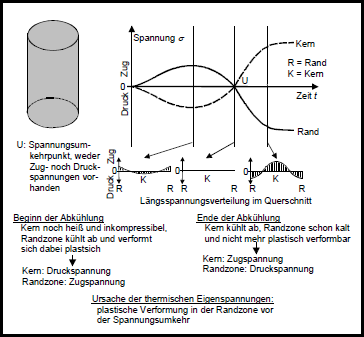
\includegraphics[scale=1.53] {eigenspanabk}
  \caption{Zeitliche Änderung der Längsspannungsverteilung im Querschnitt eines Zylinders bei schneller Abkühlung.}
  \label{fig:eigenspanabk}
  \end{figure}

\item \emph{Verformungseigenspannungen} (siehe \fref{fig:eigenspanfaser} und \fref{fig:eigenspandrahtzieh})\footcite[34]{hu} welche durch inhomogene Verformung auf Grund äußerer Beanspruchung verursacht werden.\begin{figure}[!htb]
  \centering
  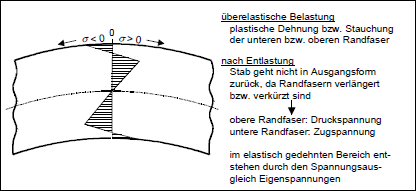
\includegraphics[scale=1.3]{eigenspanfaser}
  \caption{Schematische Längseigenspannungsverteilung im Querschnitt eines Stabs nach plastischer Biegebeanspruchung.}
  \label{fig:eigenspanfaser}
  \end{figure}
  \begin{figure}[!htb]
  \centering
  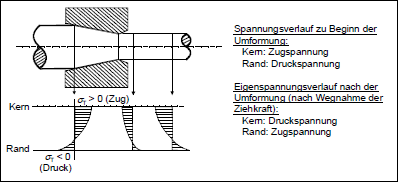
\includegraphics[scale=1.35] {eigenspandrahtzieh}
  \caption{Schematische Tangentialeigenspannungsverteilung beim Drahtziehen in Abhängigkeit von der Ziehdüsenentfernung.}
  \label{fig:eigenspandrahtzieh}
  \end{figure}
\item \emph{Umwandlungseigenspannungen} (siehe \fref{fig:eigenspanmol})\footcite[35]{hu} die durch inhomogene Gefügeumwandlungen  
mit einer einhergehenden Volumenänderung ausgelöst werden.\begin{figure}[!htb]
  \centering
  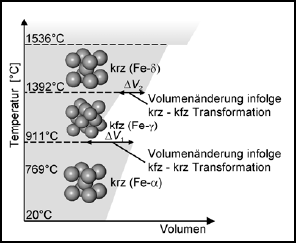
\includegraphics[scale=1.867] {eigenspanmol}
  \caption{Volumenänderung durch Veränderung der Gitterstruktur.}
  \label{fig:eigenspanmol}
  \end{figure}
\end{itemize}

Bei dem Messen von Eigenspannungen wird in zerstörende sowie zerstörungsfreie Erfassungsmethoden unterschieden. Hier wird hauptsächlich auf die zerstörenden Verfahren eingegangen und unter den zerstörungsfreien nur die Finite-Elemente-Methode kurz erläutert. Für zylindrische Bauteile werden Ausbohr- und Abdrehverfahren verwendet um die Eigenspannungen in radialer, tangentialer sowie axialer Richtung zu erfassen.Die Eigenspannungen in Platten und Stäben werden mit schichtweisem Abtragen, Einschneiden und Aufschlitzen ermittelt.\begin{figure}[!htb]
  \centering
  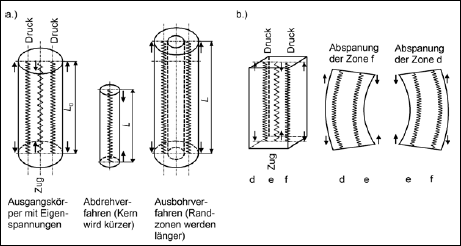
\includegraphics[scale=1.1] {eigenspanschnitt}
  \caption{Ermittlung von Eigenspannungen a) in zylindrischen Bauteilen und b) in Platten und Stäben.}
  \label{fig:eigenspanschnitt}
  \end{figure}
  Nach der jeweiligen Entfernung des Materials lassen sich Bauteilgeometrieänderungen sehr gut erkennen oder auch mit Messgeräten erfassen und daraus  sind Schlüsse auf die Art und Lage der spezifischen Eigenspannungen abzuleiten (siehe \fref{fig:eigenspanschnitt})\footcite[36]{hu}. Zur ganz präzisen Analyse  und Visualisierung von Bauteilspannungen kommt heutzutage in der Industrie  die FEM (Finite-Elemente-Methode zum Einsatz).\footcite[Vgl.][32-37]{hu} Mit ihr lassen sich Umformprozesse sehr gut simulieren. Die FEM ist ein numerisches Verfahren zur näherungsweisen Lösung kontinuierlicher Feldprobleme. Darunter versteht man Probleme, in denen das Verhalten des Kontinuums durch partielle, orts- und zeitabhängige Differentialgleichungen umschrieben wird. Für jede Zustandsgröße eines Kontinuums gehören unendlich viele Werte, weil sie eine Funktion jedes Punktes des Kontinuums beschreibt. Die FEM zerlegt das Kontinuum in \emph{endlich} viele Teile, die sogenannten \emph{finiten Elemente}. Ein komplexes, kontinuierliches Problem wird dabei in eine endliche Zahl einfacher, voneinander abhängiger Probleme unterteilt.\footcite[Vgl.][48]{fu}
\subsection{Umformgrad}
In der Umformtechnik wird zwischen elastischer und plastischer Formänderung unterschieden. Bildet sich ein Körper nach einer Deformation vollständig zu seiner ursprünglichen Geometrie zurück so ist er in dem elastischen Bereich gedehnt worden. Wird ein Bauteil über diesen Bereich hinaus gedehnt so tritt eine bleibende Verformung ein, was man unter plastifizierten Zustand versteht.  Bei herkömmlichen einachsigen Zug- oder Druckversuchen werden Spannung und Dehnung auf Ihre Ausgangsgrößen bezogen z.B. \begin{equation}\sigma=\frac{F}{A_o}\end{equation} oder für die Dehnung \begin{equation}\varepsilon = \frac{\Delta l}{l_0}\end{equation} Diese Methode der Festigkeitsberechnung ist für Bauteile die konstruktionsbedingt für den elastischen Bereich dimensioniert werden   durchaus ausreichend. In der Umformtechnik sind aber die \emph{wahren Spannungs- und Dehnungsverhältnisse} von großer Bedeutung. Die wahre Spannung, die die momentan einwirkende Kraft auf die momentane Fläche bezieht ist die \emph{Fließspannung} $ k_f $. Für die \emph{wahre Dehnung} die den eigentlichen Umformgrad $ \varphi $ darstellt bezieht sich auf den sich mit der Verformung ändernden Bezugswert. Eine Herleitung die z.B. bei einem einachsigen zylindrischen Druckversuch in dem der Höhenunterschied \begin{equation}
h=h_1-h_0 \end{equation}  den zurückgelegten Stempelweg darstellt ist:\begin{equation}
\varphi=\int\limits_{h_0}^{h_1}\frac{dh}{h}=\ln h_1 - \ln h_0 = \ln\frac{h_1}{h_0}\end{equation} Im Falle des Druckversuchs ergibt sich dafür natürlich ein negativer Umformgrad. Erwähnt werden sollte in diesem Zusammenhang noch das Gesetz der \emph{Volumenkonstanz} welches aussagt das  bei plastischen Fließvorgängen das Volumen des Kontinuums unverändert bleibt. So kann man den Stauchvorgang eines Vierkantstabes so beschreiben: 






 \begin{equation}h_1 \cdot  b_1 \cdot l_1 = h_0 \cdot b_0 \cdot l_0\end{equation} 
Nach Transformation und Logarithmieren der Gleichung erhält man
das Gesetz der Volumenkonstanz. 
 
 
 \begin{equation}\ln (\frac{h_1}{h_0} \cdot \frac{b_1}{b_0} \cdot \frac{l_1}{l_0}) = \ln 1 = 0\end{equation} 
 
daraus folgt \begin{equation}
\ln\frac{h_1}{h_0}+\ln\frac{b_1}{b_0}+\ln\frac{l_1}{l_0}=\varphi_1+\varphi_2+\varphi_3=0
\end{equation}
Analog dazu gilt für die Umformgeschwindigkeiten
\begin{equation}
\dot{\varphi_1}+\dot{\varphi_2}+\dot{\varphi_3}=0
\end{equation}

Durch den hydrostatischen Spannungsanteil beschriebene Dehnungen und Dehngeschwindigkeiten werden bei plastischen Fließvorgängen gleich null.\footcite[Vgl.][24-28]{fu}
\subsection{Umformgeschwindigkeit}
An dieser Stelle soll die bei Umformprozessen auftretende Geschwindigkeit hergeleitet werden. Man erhält sie aus der zeitlichen Ableitung des Umformgrades
\begin{equation}
\dot{\varphi} = \frac{\text{d}\varphi}{\text{d}t}
\end{equation}
Man nehme zum Beispiel den klassischen Stauchversuch und geht davon aus, dass der Umformgrad $ \varphi $ eine Funktion der Probenhöhe (Probe ist meist ein zylindrischer Körper) $ h $ ist während die Höhe $ h $ auch eine Funktion der Zeit $ t $ darstellt. Daraus kann folgender Term geformt werden 
\begin{equation}
\frac{\text{d}\varphi}{\text{d}t} = \frac{\text{d} \varphi (h(t))}{\text{d}t}= \frac{\text{d}\varphi}{\text{d}h} \cdot \frac{\text{d}h}{\text{d}t}
\end{equation}
Hieraus folgt für den einachsigen Spannungszustand mit der jeweiligen Werkzeuggeschwindigkeit (hier der Stempel) $ v $ sowie der Probenhöhe $ h $
\begin{equation}
\dot{\varphi}=\frac{\text{d}\varphi}{\text{d}t}= \frac{\text{d}(\ln h - ln  \, h_0)}{\text{d}h}\cdot \frac{\text{d}h}{\text{d}t} = \frac{v}{h}
\end{equation}
Wobei $ h_0 $ natürlich die Ausgangshöhe der Probe ist.\footcite[Vgl.][65]{hu}
Aus diesen Ausführungen lässt sich schließen,  dass die Umformgeschwindigkeit immer aus der im Augenblick aufgenommenen Werkzeuggeschwindigkeit und der zum gleichen Zeitpunkt erfassten Bauteilhöhe (oder auch dem jeweiligen Umformvorgang spezifischem   Maß) gebildet wird.
\subsection{Einachsiger Spannungszustand}
Zum Grundlagenverständnis soll nun das Spannungsverhältnis des einachsigen Spannungszustandes an einem einfachen Zugstab erläutert werden (siehe \fref{fig:einachsspann})\footcite[Vgl.][388]{dd}\begin{figure}[hbtp]
\centering
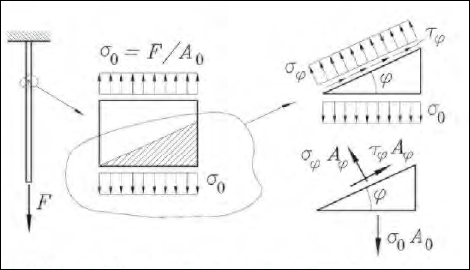
\includegraphics[scale=1.14]{einachsspann}
\caption{Einachsiger Spannungszustand am Zugstab}
\label{fig:einachsspann} 
\end{figure}
Bei Belastung eines Bauteils in nur einer Richtung liegt der sogenannte einachsige Spannungszustand vor. Wenn man an dem Zugstab \fref{fig:einachsspann} einen Schnitt nicht senkrecht zur Richtung von $ \sigma_0 $ betrachtet, erkennt man, dass dort auch Schubspannungen im Bauteil vorhanden sind. Um einen Gleichgewichtszustand in horizontaler Richtung an dem herausgeschnittenen Keil herzustellen ist es nötig das in der schrägen Schnittfläche $ A_{\varphi} $ außer der Nomalspannung $ \sigma_{\varphi} $ zusätzlich die Schubspannung $ \tau_{\varphi} $ vorhanden ist. Durch Multiplikation der Spannungen in den Schnittflächen $ A_0 $ und $ A_{\varphi} $ mit den entsprechenden Flächen erhält man die Kräfte $ \sigma_0\A_0 $ und $ \sigma_{\varphi}A_{\varphi} $. Es können nun fogende Gleichgewichtsbedingungen aufgestellt werden \begin{equation}
\sigma_{\varphi}A_{\varphi} - \sigma_0 A_0\cos{\varphi} = 0 \end{equation}
\begin{equation}
\tau_{\varphi}A_{\varphi} - \sigma_0A_0\sin{\varphi} = 0
\end{equation} Durch Einsetzten von $ A_0 = A_{\varphi}\cos{\varphi}$ erhält man die Gleichungen für die Spannungen in einem beliebigen Schnitt bei dem einachsigen Spannungszustand
\begin{equation}
\sigma_{\varphi} = \sigma_0\cos^2{\varphi}
\end{equation}
\begin{equation}
\tau_{\varphi} = \frac{1}{2} \sigma_0\sin{2\varphi}
\end{equation}
Aus diesen Gleichungen ist zu erkennen das die Normalspannung am größten bei $ \varphi = 0 $ ist, weil in dem Schnitt keine Schubspannung vorhanden ist. Deshalb wird $ \sigma_0 $ in diesem Fall als \emph{Hauptspannung} bezeichnet. Die maximale Schubspannung ergibt sich bei $ \varphi = 45^{\circ} $ sie wird als \emph{Hauptschubspannung} ($ \tau_{\text{max}} = \frac{1}{2}\sigma_0 $ ) bezeichnet.\footcite[Vgl.][388]{dd}



  
\subsection{Spannungsvektor und Spannungstensor}
Zum besseren Verständnis was für Kräfte und Spannungsverhältnisse bei Umformvorgängen im Material vorherrschen ist es sinnvoll sie an infinitesimal kleinen Volumenelementen zu modellieren. Dazu stellt man sich einen Körper unter Belastung der Einzelkräfte $ F_i $ und der Flächenlasten $ p $ \ vor ( siehe \fref{fig:normalvektor}) \footcite [Vgl.][43]{tmr}. Äußere Belastungen verursachen grundsätzlich auch innere Kräfte in einem Bauteil. Betrachtet man den Schnitt s--s \begin{figure}[!htb]
  \centering
  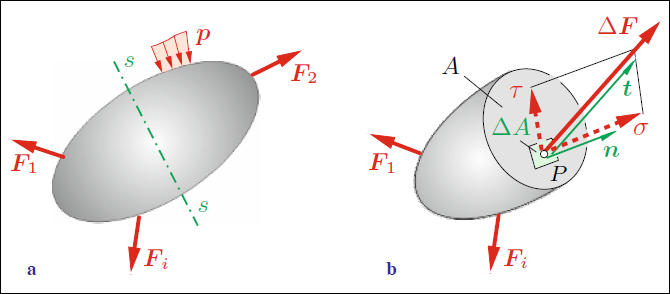
\includegraphics[scale=.8] {normalvektor}
  \caption{Spannungsvektor an beliebigen Körper}
  \label{fig:normalvektor}
  \end{figure} erkennt man das die inneren Kräfte sowie Spannungen über die ganze Schnittfläche $ A $ verteilt sind. Spannung sind über die Schnittfläche veränderlich deshalb  wird ein beliebiger Punkt $ P $ der Schnittfläche definiert. Die Schnittkraft $ \Delta F $  wirkt auf ein Flächenelement $ \Delta A $ (in dem $ P $ enthalten ist). Es wirkt eine gleich große entgegengesetzte Kraft auf die gegenüberliegende Schnittfläche (actio gleich reactio). Der Quotient $ \frac{\Delta F}{\Delta A} $ (Kraft auf die Fläche bezogen) definiert die mittlere Spannung für das Flächenelement. Wenn man nun bei der Beziehung $ \frac{\Delta F}{\Delta A} $ den Differentialquotienten bildet in dem $ \Delt A \rightarrow 0 $ gegen Null läuft  resultiert daraus die Formel für den \emph{Spannungsvektor }$ t $ \begin{equation} t = \lim \limits_{\Delta A \to 0} \frac{\Delta F}{\Delta A} = \frac{\text{d}F}{\text{d}A} \end{equation}
Der Spannungsvektor lässt sich in eine Komponente normal zur Schnittfläche ( \emph{Normalspannung} $ \sigma $) und eine Komponente in der Schnittfläche (tangentiale \emph{Schubspannung} $ \tau $) zerlegen. Es existiert eine Abhängigkeit des Spannungsvektors $ t $ von der Lage des Punktes $ P $ in der Schnittfläche. Also eine Ortsabhängigkeit. Kann der Spannungsvektor $ t $ für alle Punkt von A angegeben werden, so ist die Spannungsverteilung in der Schnittfläche bekannt. Dennoch wird durch $ t $ der Spannungszustand in einem Punkt $ P $ nicht vollständig definiert. Werden durch $ P $ Schnitte in verschiedene Richtungen gelegt, so wirken entsprechend der unterschiedlichen Orientierung der Flächenelemente auch unterschiedliche Schnittkräfte. Es liegt demzufolge auch eine Schnittrichtungsabhängigkeit der Spannungen vor. Die Schnittrichtung wird von dem Normalenvektor $ n $ charakterisiert. Der Spannungszustand in einem Punkt $ P $ wird durch drei Spannungsvektoren in drei senkrecht aufeinander stehenden Schnittflächen festgelegt. Zu Darstellungszwecken fallen die drei Schnittflächen in dieser Modellierung mit den Koordinatenebenen eines kartesischen Koordinatensystems zusammen.

Um sie prägnant darzustellen, visualisiert man sie als Seitenflächen eines infinitesimalen Quaders mit den Kantenlängen d$ x $, d$ y $ und d$ z $ in der Umgebung von $ P $\begin{figure}[!htb]
  \centering
  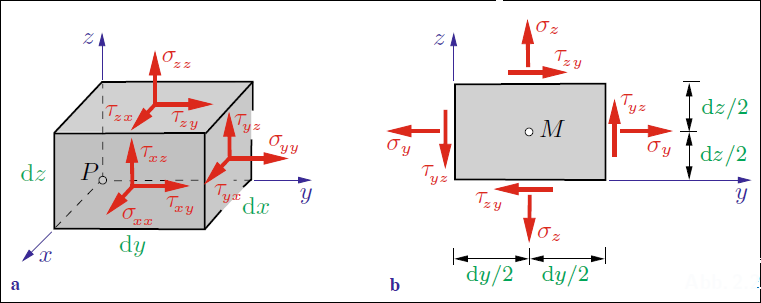
\includegraphics[scale=.7] {tensor}
  \caption{Spannungen und Kräfte am Infinitesimalelement}
  \label{fig:tensor}
  \end{figure}( siehe \fref{fig:tensor})\footcite[Vgl.][44]{tmr} . Ein Spannungsvektor wirkt hier je Fläche, der in seine Komponenten senkrecht zur Schnittfläche (daraus folgt Normalspannung) und in der Schnittfläche (daraus folgt Schubspannung) zerlegt wird. Zusätzlich werden die Schubspannungen noch in die Komponenten der Richtung der Koordinatenachsen zerlegt. Es werden Doppelindizes zur Kennzeichnung der jeweiligen Komponenten benutzt(siehe \fref{fig:tensor}). 
Der erste Index kennzeichnet die Richtung der Flächennormalen, wohingegen der zweite Index die Richtung der Spannungskomponenten bezeichnet. Zum Beispiel deklariert $ \tau_{yx} $ die Schubspannung einer Ebene, deren Normale in $y$ - Richtung weist. Die Spannung zeigt hier in die $ x $ - Richtung (siehe \fref{fig:tensor}). Es ist sinnvoll und vermeidet Verwechselungen bei den Normalspannungen die Schreibweise zu simplifizieren. Spannung und Flächennormale besitzen in diesem Fall die gleiche Richtung. Daraus ergibt sich eine Übereinstimmung der beiden Indizes und es ist hinreichend nur einen Index anzugeben. Es ist also völlig ausreichend  folgende Angaben zu machen: $ \sigma_{xx} = \sigma_{x} $, $ \sigma_{yy} = \sigma_y $, $ \sigma_{zz} = \sigma_z $.

Der Spannungsvektor für die Schnittfläche, deren Normale in $ y $ - Richtung zeigt wir mit den oben angeführten Konventionen zu folgender Formel:
\begin{equation}
t = \tau_{yx}e_x + \sigma_ye_y + \tau_{yz}e_z
\end{equation}

Analog zu den Schnittgrößen existiert für die Spannungen eine \emph{Vorzeichenkonvention}:

"`\emph{Positive} Spannungen zeigen an einem positiven (negativen) Schnittufer in die positive (negative) Koordinatenrichtung."'\footcite[45]{tmr}

Infolgedessen beanspruchen positive (negative) Normalspannungen den infinitesimalen Quader auf Zug (Druck). Nach Zerlegung der Spannungsvektoren in ihre Komponenten erhält man drei Normalspannungen ($ \sigma_x$, $ \sigma_y $, $ \sigma_z $) und sechs Schubspannungen ( $ \tau_{xy}, \tau_{xz}, \tau_{yx}, \tau_{yz}, \tau_{zx}, \tau_{zy} $), die jedoch nicht alle unabhängig voneinander sind. Um das zu beweisen wird das Momentengleichgewicht um eine zur $x$- Achse parallele Achse durch den Mittelpunkt des Quaders (siehe \fref{fig:tensor})aufgestellt. Unter der Berücksichtigung das Gleichgewichtsaussagen nur für Kräfte gelten, werden die Spannungen mit den zugeordneten Flächenelementen multipliziert.
\begin{equation}
\overset{\curvearrowleft}{M}: 2\,\frac{\text{d}y}{2}\,(\tau_{yz}\,\text{d}x\,\text{d}z) - 2\,\frac{\text{d}z}{2}\,(\tau_{zy}\, \text{d}x\,\text{d}y)\,= 0 \Rightarrow\,\tau_{yz} = \tau_{zy}
\end{equation} Analog dazu gilt für die anderen Achsen: \begin{equation}
\tau_{xy}=\tau_{yx},\quad\tau_{xz}=\tau_{zx},\quad\tau_{yz}=\tau_{xy}
\end{equation}

Aus dem folgt:

"`Schubspannungen in zwei senkrecht aufeinander stehenden Schnitten (z.B. $\tau_{xy}$ und $\tau_{zy}$) sind gleich."'\footcite[46]{tmr}

Sie werden als einander \emph{zugeordnete Schubspannungen} bezeichnet. Aufgrund der Tatsache das sie gleiche Vorzeichen besitzen, deuten sie entweder auf die gemeinsame Quaderkante oder sie sind beide von ihr abgewandt. Wie aus den oben angeführten Identitäten zu erkennen ist, existieren lediglich sechs unabhängige Spannungen. Die Komponenten der jeweiligen Spannungsvektoren lassen sich in einer Matrix anordnen:
\begin{equation}
\sigma = \begin{pmatrix}
\sigma_x & \tau_{xy} & \tau_{xz}\\
\tau_{yx} & \sigma_y & \tau_{yz}\\
\tau_{zx} & \tau_{zy} & \sigma_z
\end{pmatrix} = \begin{pmatrix}
\sigma_x & \tau_{xy} & \tau_{xz}\\
\tau_{xy} & \sigma_y & \tau_{yz}\\
\tau_{xz} & \tau_{yz} & \sigma_z
\end{pmatrix}
\end{equation}

Die Normalspannungen bilden die Hauptdiagonale. Alle anderen Elemente sind Schubspannungen. Die Matrix ist symmetrisch und stellt den \emph{Spannungstensor} dar. Er wird mit der Größe $ \sigma $ bezeichnet. Der \emph{Spannungszustand} wird durch den \emph{Spannungstensor} (Spannungsvektoren für drei aufeinander stehende Schnitte) eindeutig in einem Punkt festgelegt.\footcite[Vgl.][43-46]{tmr}
\subsubsection{Festigkeitshypothesen}
In der Praxis unterliegen Bauteile nahezu immer einem mehrachsigen Spannungszustand. Zulässige Spannungen $ \sigma_{zul} $ für Bauteile und Werkstoffe werden aber meistens mit dem einachsigen Zugversuch in Laboren festgelegt. Um nun die realen Spannungsverhältnisse im Bauteil mit den Laborwerten vergleichbar zu machen bedient man sich bestimmter Festigkeitshypothesen, die die Hauptspannungen berücksichtigen um sie mit den theoretischen Mindestzugfestigkeiten gegenüberzustellen. Es wird also zuerst unter zu Hilfenahme einer Spannungshypothese eine Vergleichsspannung $ \sigma_V $ errechnet  und diese dann mit $ \sigma_{zul} $ verglichen. Idealisiert würde solch eine Vergleichsspannung alle wirkenden Veränderungen und Spannungen sowie Veränderungen des Materialverhaltens (z.B. Fließen, Bruch) bei gleichen Werten auslösen wie im einachsigen Spannungszustand bei dem modellierten Zugversuch. Bei der Gegenüberstellung der beiden Spannungen gilt dann $ \sigma_V \leq \sigma_{zul} $. Es wurden im laufe der Jahre zahlreiche solcher Spannungshypothesen hergeleitet.\footcite[Vgl.][399]{dd} Hier sollen nur die geläufigsten, nämlich die Spannungshypothesen von  \emph{Tresca} und \emph{von Mises} kurz vorgestellt werden.

Die \emph{Schubspannungshypothese} nach Tresca geht davon aus, dass die Materialbeanspruchung durch die maximale Schubspannung zu charakterisieren ist. Für den dreidimensionalen Spannungszustand gilt die Formel \begin{equation} \sigma_V = \sqrt{(\sigma_x - \sigma_y )^2 + 4\tau^2_{xy}} \end{equation}. Bei der \emph{Hypothese der Gestaltänderungsenergie} nach von Mieses wird davon ausgegangen, dass die zur Änderung der Gestalt benötigte Energie zu Vergleichszwecken herangezogen wird. Für den räumlichen Spannungszustand wird folgernder Term gegeben: \begin{equation} \sigma_V = \sqrt{\sigma^2_x + \sigma^2_y - \sigma_x\sigma_y + 3\tau^2_{xy}} \end{equation} 
Die Hypothese der Gestaltänderungsenergie ist besonders bei zähen Werkstoffen aussagekräftiger und präziser als die Schubspannungshypothese.\footcite[Vgl.][84]{tmr}















  
\newpage
\section{Bauteil}
Prüfobjekt ist in den folgenden Untersuchungen der Verdeckkastendeckel  des Audi A3 Cabriolet's (siehe \fref{fig:audia3}).
 Als Verzierung eines Luxusobjektes sind die Anforderungen an Aussehen und Qualität außergewöhnlich hoch. So dient er zum einen als rein optisches Veredelungselement zum anderen hat er auch funktionelle Aufgaben (z.B. Stabilität in den gesamten Kofferraumdeckel bringen oder auch als Antenne zu agieren). Geringe Spaltmaße,  perfekte Symmetrie (das menschliche Auge erkennt ein Hundertstel Millimeter) so wie allgemeine Benutzerfreundlichkeit (z.B. Hängenbleiben von Kleidungsstücken und Ähnlichem an dem Verzierungsobjekt sollte ausgeschlossen sein) sind Anforderungen die höchste Priorität haben.
 Darüber hinaus sind  flüssige Übergänge und Einklang   zu weiteren Verzierungselementen des Fahrzeuges von großer Bedeutung für einen harmonischen Gesamteindruck.
 
   
\begin{figure}[!htb]
\centering
\hfill
\subfloat[Audi A3 ]{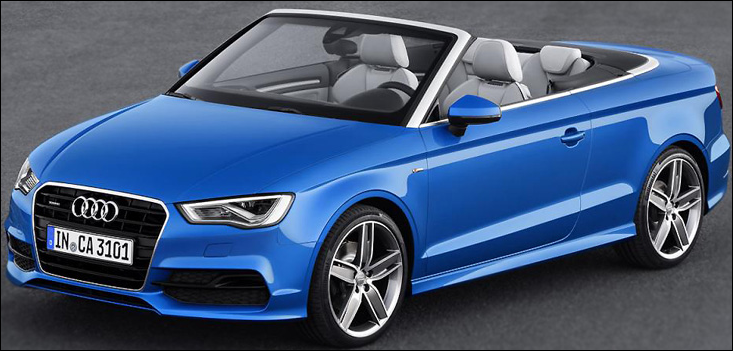
\includegraphics[scale=.4667]{audia3blau}}
\hfill
\subfloat[Audi A3 Verdeckkastendeckel \label{fig:audia3verdeck}]{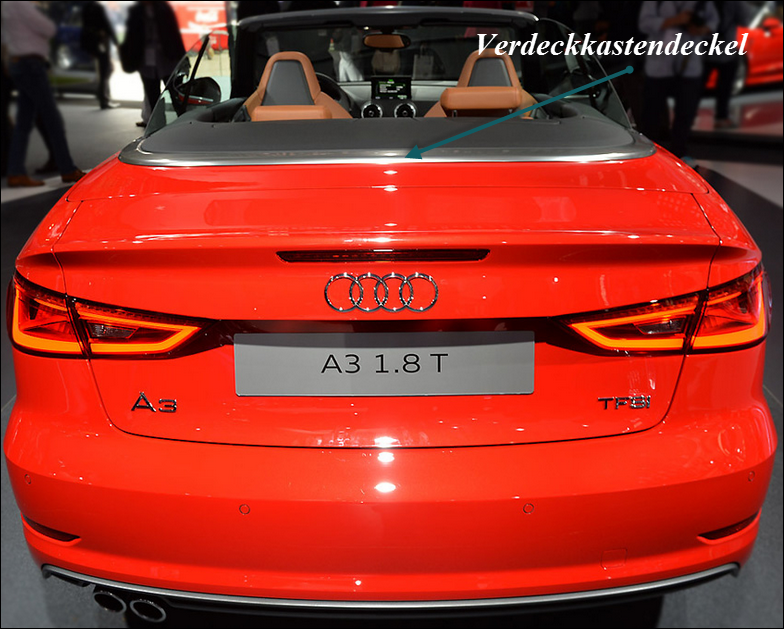
\includegraphics[scale=.263]{audivdkd}}
\hfill
\caption[Audi A3 Endprodukt]{Audi A3 Endprodukt\footnotemark }
\label{fig:audia3}
\end{figure}
 \footnotetext{Vgl.http://www.cars.co.za/motoring\_news/2014-audi-a3-cabriolet-completes-the-a3-family/6061/[28.12.2013].}



	 	 
\subsection{Funktion \& Qualitätsumfang}
An Verzierungselemente werden gerade in der Automobil Oberklasse besonders hohe Ansprüche gestellt. Es sind besonders folgende hervorzuheben:
\begin{itemize}
\item keine Beulen
\item keine Oberflächenfehler
\item ideale Fugenläufe
\item präzise Radien
\item enge Form- und Lagetoleranzen (siehe \fref{fig:vdkdtol})
\item enge Spalttoleranzen
\end{itemize}
\begin{figure}[!htb]
  \centering
  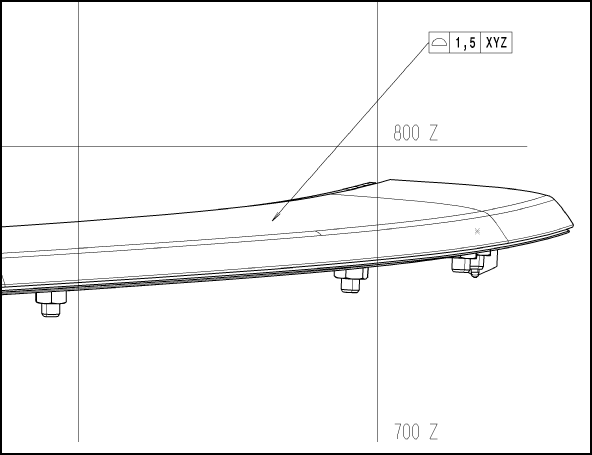
\includegraphics[width=1\linewidth,height=.2\textheight] {vdkdtol}
  \caption{Wölbungstoleranz}
  \label{fig:vdkdtol}
  \end{figure}






\subsection{Aluminium}
Aufgrund seiner geringen Dichte (\SI{2.69}{\kilo\gram\per\deci\meter\cubed})\footcite[Vgl.][353]{wm}, guten Umformbarkeit, Korrosionsbeständig und mit einer hervorragend zu erzielender Oberflächengüte sowie hohem Reflexionsgrad ist Aluminium das am häufigsten verwendete Ausgangsmaterial für Zierleisten.\\
 Es werden überwiegend Strangpressprofile verarbeitet die bei den Lieferanten mit bestimmten Eigenschaften angefordert werden. Die wichtigsten dort angeführten mechanischen Eigenschaften sind die Zugfestigkeit $R_m  [\si{\newton\per\milli\meter\squared}$], Dehnung $R_{po,2} [\si{\newton\per\milli\meter\squared}]$,   Bruchdehnung A oder auch $A_{50} [\si{\percent}]$ (der Index 50 bezieht sich auf eine Messlänge  von \SI{50}{\milli\meter} der Probe  beim einachsigen Zugversuch)\footcite[Vgl.][281]{aa}und die Korngröße.\\
  Sie wird in der Einheit [\si{\micro\meter\squared}] angegeben und hat Einfluss auf die Oberflächengüte nach  Umformprozessen. Bei steigendem Umformgrad ergibt sich häufig eine Aufrauung der Oberfläche (Orangenhaut)\label{sec:orangenhaut} die von der Ausgangskorngröße abhängig ist. Je geringer die Ausgangskorngröße desto geringer der Aufrauungseffekt.\footcite[Vgl.][524]{aa}\\ Stark verformtes und grobkörniges Material entwickelt oft in den deformierten Zonen (insbesondere in den gestreckten Bereichen) eine Oberflächenrauigkeit (Orangenhaut), die die Reflektivität und Einfärbbarkeit des Endproduktes stark einschränkt. Das Phänomen \emph{Orangenhaut} entsteht vorwiegend an Umformbereichen die nicht in direktem Kontakt mit Werkzeugoberflächen stehen.\footcite[Vgl.][19]{hmp}
Erwähnenswert ist zu Vorangegangenem noch, dass aufgrund der bei den meisten Aluminiumlegierungen, nicht ausgeprägten Streckgrenze  die $R_{p0,2}$ Dehngrenze als Bemessungskennwert bei einer \SI{0.2}{\percent} bleibenden Verformung gegenüber rein elastischem Verhalten ermittelt wird (siehe \fref{fig:spanndehn2}).\footcite[Vgl.][280-281]{aa}  
\begin{figure}[h!tbp]
\centering
 	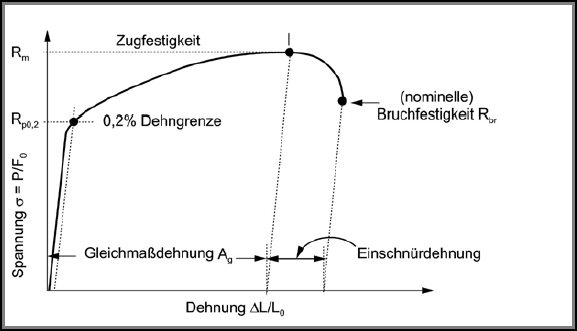
\includegraphics[scale=1.05]{spanndehn2}
 	\caption{Spannungs-Dehnungs Schaubild mit $Rp_{0,2} $ Dehngrenze}
 	\label{fig:spanndehn2}
 	\end{figure}
	 	 	 	 
	 	 	 	 

\subsection{Streckbiegen}
Unter Biegen versteht man nach DIN 8586 das Umformen von festen Körpern, wobei der plastische Zustand im Wesentlichen durch eine Biegebeanspruchung herbeigeführt wird.\footcite[Vgl.][376]{hu} Die Blechumformung verfolgt generell das Ziel aus einem Flachprodukt ein räumliches Gebilde zu formen, ohne dabei (im Idealfall) die Blechdicke zu verändern.  Eine Formänderung vollzieht sich aus diesem Grunde hauptsächlich in der Blechebene unter ebenem Spannungszustand. Als Grundverfahren in der Blechumformung sind Verfahren wie Tiefziehen, Biegen und Streckziehen (oder auch Streckbiegen) zu nennen. Gemeinsam haben sie alle, dass sich Stauch- und Streckverformungen in der Blechebene und Blechdicke abspielen und unterschiedliche Dehnungszustände und -abläufe anzutreffen sind.\\ Die Umformbarkeit (Duktilität) als Werkstoffeigenschaft ist wegen der Tatsache, dass  Spannungs- und Dehnungszustände mit den Fließ- und Brucheigenschaften eines Werkstoffes in Wechselwirkung stehen, ein komplexes Gebiet. Über das Werkzeugsystem (Stempel, Niederhalter etc.) werden die benötigten Umformkräfte in das Werkstück eingeleitet und erwirken so über die  Formänderungen, Relativbewegungen zwischen Werkzeug und Werkstück bei veränderlichen Anpreßkräften. Die zwischen Bauteil (Werkstoff) und Wirkteil (Werkzeug z.B. Stempel) entstehenden Reibungsverhältnisse resultieren aus den  Grenzflächen- und Gleiteigenschaften von Wirkteil und Werkstoff.\\ Insbesondere bei Aluminiumwerkstoffen haben sie bedeutenden Einfluss auf das Umformergebnis. Der Werkzeugaufbau und die Werkzeuggeometrien so wie die Steuerung des Fertigungsvorgangs haben erheblichen Anteil an der Art und Weise des Werkstoffflusses bei den Biegeprozessen.\footcite[Vgl.][499]{aa}
Bei dem Umformverfahren Streckbiegen werden auf speziellen Streckbiegemaschinen die Enden eines Profilstranges in Spannern gehalten und auf  Zugspannung gebracht (siehe  \fref{fig:Streckbiegemaschine}). Anschließend werden sie über ein massives Biegewerkzeug streckgebogen.\footnote{Vgl.\url{http://www.tillmann-gruppe.de/de/streckbiegen.html}[27.10.2013].} 
\begin{figure}[!htb]
\centering
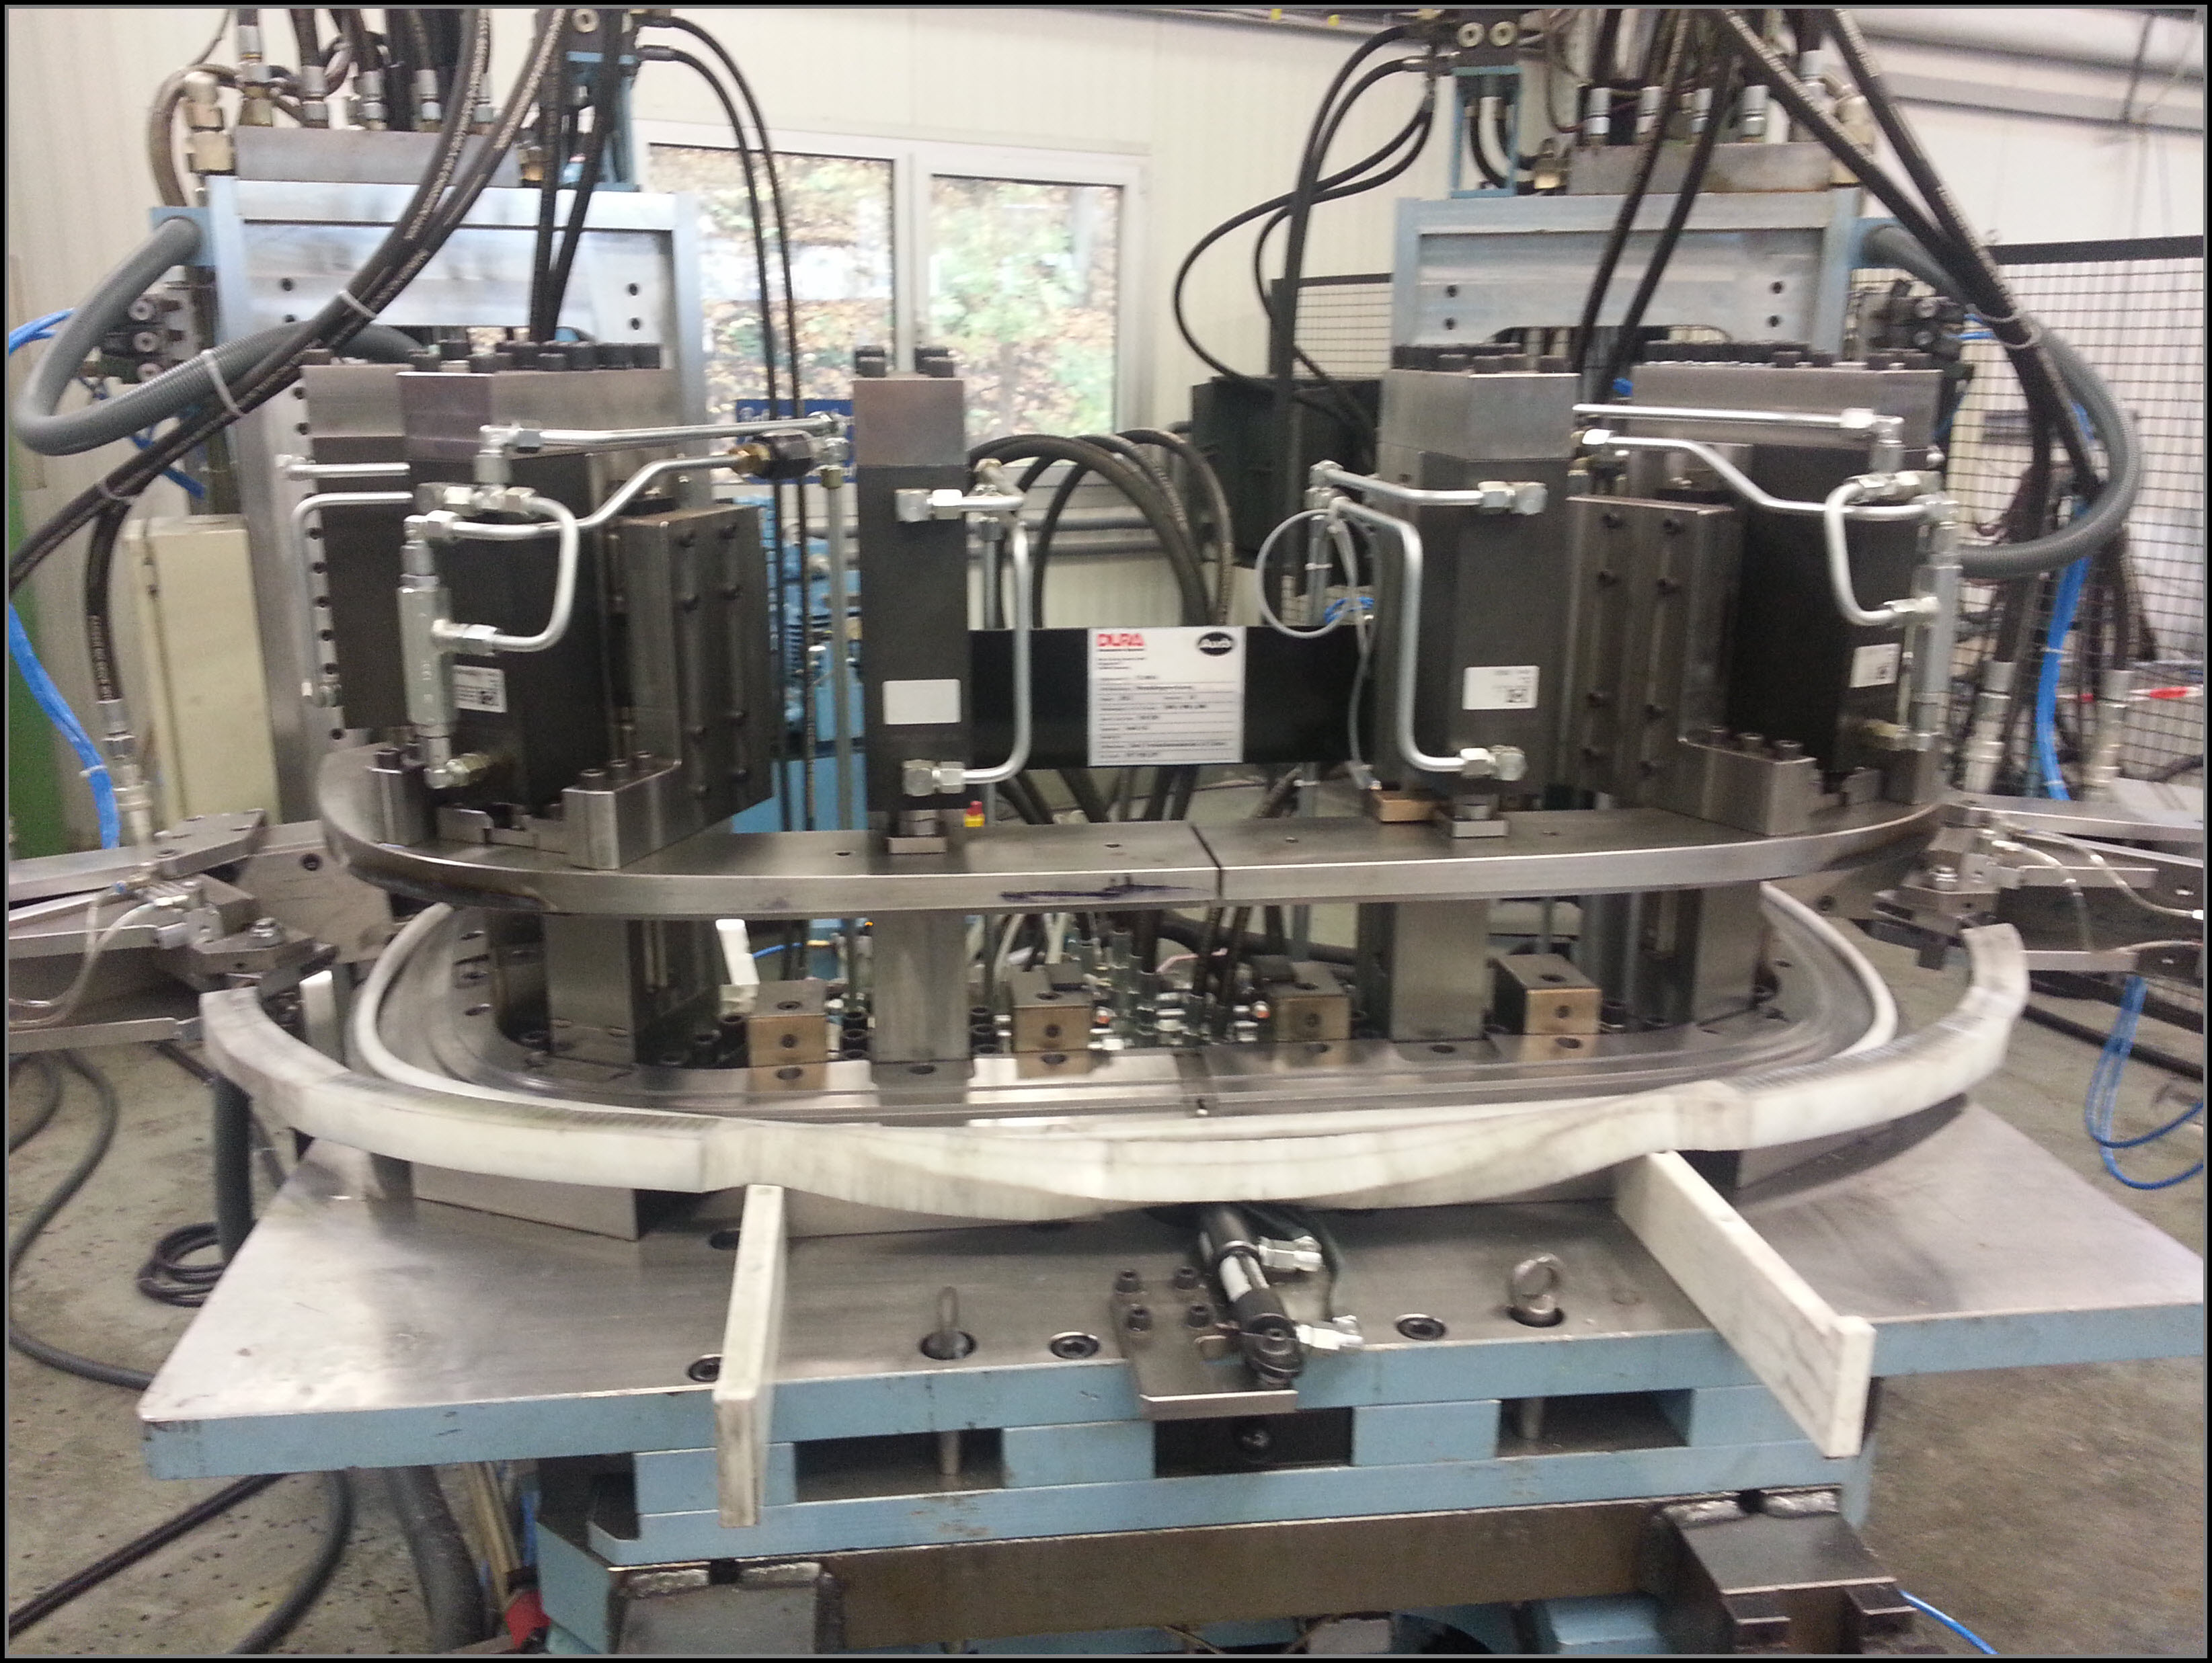
\includegraphics[scale=.12]{Streckbiegemaschine}
\caption{Streckbiegemaschine}
\label{fig:Streckbiegemaschine}
\end{figure}
Das Streckbiegeverfahren was bei der Firma DURA  für den Verdeckkastendeckel des Audi A3 eingesetzt wird ähnelt mehr dem \emph{Tangentialstreckziehen}. Der Unterschied zu dem herkömmlichen Streckziehen das in einer Arbeitsstufe erfolgt und bei dem die Zugspannung nur über den Stempel eingeleitet wird ist das Fertigen in zwei Arbeitsschritten.

 Im ersten Schritt wird das Strangpressprofil in die Spannvorrichtung der Steckbiegemaschine eingelegt und an den Enden eingespannt. Danach fahren die Spannelemente horizontal auseinander und leiten eine Zugspannung in das Bauteil ein. Es wird knapp über den Bereich der Streckgrenze gestreckt. Je nach Material und erwünschtem Biegeresultats werden die aufgewandten Zugkräfte von den Maschineneinrichtern präzise eingestellt.\\
  Im zweiten Schritt erfolgt nun die eigentliche Formgebung. Das gestreckte Strangpressprofil wir unter Aufrechterhaltung der eingebrachten Zugspannung mit einer kontinuierlichen Geschwindigkeit tangential um das formgebende Wirkteil gelegt. Die Bewegung wird von den Spannelementen alleinig ausgeführt (siehe \fref{fig:streckbiegen})\footnote{\url{http://www.custompartnet.com/wu/sheet-metal-forming}[04.02.2014].}. 
  \begin{figure}[hbtp]
  \centering
  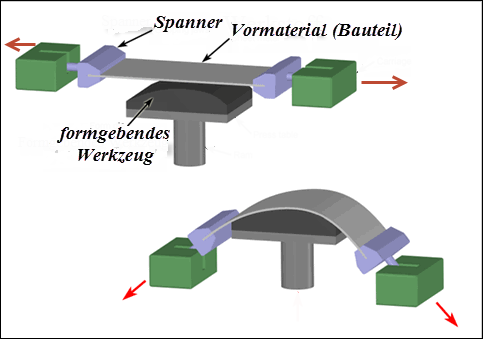
\includegraphics[scale=1.1]{streckbiegen}
  \caption{Prinzip Streckbiegen}
  \label{fig:streckbiegen} 
  \end{figure}
  
Das Ausgangsmaterial (Aluminium Strangpressprofile) wird streckgebogen um eine Rückfederung (siehe \fref{fig:springback})\footcite[Vgl.][65]{smfpd} zu minimieren.  Die Rückfederung entsteht aus der Rückbildung der elastischen Formänderung des Bauteils nach der Beendigung des Biegevorgangs und nach dem Entfernen der eingeleiteten Kräfte. Es findet im Werkstoff eine elastische Erholung statt. In der Blechmanufaktur und Blechumformung stellt die Rückfederung eine der bedeutendsten Formgebungsproblematiken dar.
\\
 Sie ist ein äußerst komplexes Phänomen da sie von mannigfaltigen Interaktionen zwischen den Materialeingenschaften, der Bauteilgeometrie, der Reibung,  der Werkzeugradien und weiteren formgebenden Bedingungen abhängt. Unter den Variablen, die die Rückfederung verringern sind der Reibungskoeffizient und die Reibung, die Streckkraft, die Nachbiegekraft, die Formänderungsgeschwindigkeit, die Temperatur sowie weitere geometrische Parameter zu bezeichnen. Hervorzuheben ist an dieser Stelle, dass das Verhältnis des Biegeradius $ R $ zur Blechdicke $ t $ in einem Bereich von $ \frac{R}{t} < 10 $ die Rückfederung wesentlich vergrößert. Im laufe der Zeit haben sich verschiedenen Methoden zur Unterdrückung der Rückfederung bewährt. Zu ihnen zählen das Überbiegen, das Strecken und das Nachdrücken oder Nachpressen. Zur Kompensation der Rückfederung hat sich das Überbiegen als das sicherste Verfahren in der Vergangenheit erwiesen. Es wird in der Fertigungspraxis davon ausgegangen das ein Überbiegungsspielraum von 2 \%  bei Stahlbauteilen ausreichend ist um Rückfederungseffekte zu minimieren.\\ Das Nachpressen in der Biegeregion hat den Nachteil, dass hohe Presskräfte aufgebracht werden müssen um einen gewünschten Effekt zu erzielen. Bei dem Verfahren  Streckbiegen zur Optimierung der Rückfederung wird das Bauteilmaterial zu erst über den Bereich der Streckgrenze hinweg (meistens durch Aufbringung hydraulischer Zugkräfte) gestreckt und dann über das formgebende Werkzeug gebogen. Dieses Verfahren wird nur bei großen Biegeradien angewandt weil kleine Radien eine sehr große Vorspannung (jenseits der Mindestzugfestigkeit) benötigen würden.\footcite[Vgl.][16-19]{hmp}\\  \begin{figure}[hbtp]
 \centering
 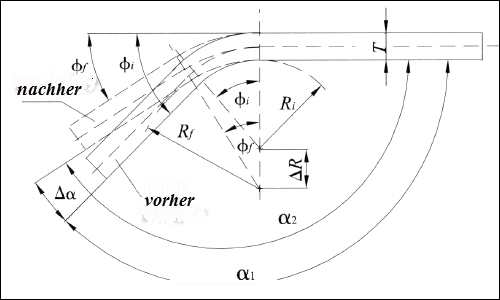
\includegraphics[scale=1]{springback}
 \caption{Prinzip der Rückfederung}
 \label{fig:springback}
 \end{figure}
Ein weiterer kritischer Punkt bei dem Verfahren Streckbiegen und Biegeprozessen generell sind die Spannungsverläufe in der Verformungszone die Eigenspannungen in das Bauteil bringen welche bei späteren Bearbeitungsverfahren wie z.B. das Beschneiden oder Fräsen in der Nähe des Deformierungsbereiches Verzug und Maßänderungen hervorrufen.\\ Je nach dem wie weit das Ausgangsmaterial über die Streckgrenze hinaus getreckt wird (bis zu welchem Grad das Material fließt) verschiebt sich die neutrale Faser in dem Biegebereich in Richtung des kleinen Radius (also nach innen). Bei sehr großer Streckung ist es möglich das die neutrale Faser sogar außerhalb des Bauteils liegt.\footcite[Vgl.][374]{fu} Bei den Versuchsreihen welche in dieser Ausarbeitung durchgeführt werden, bleibt die neutrale Faser innerhalb des Bauteils weil nur sehr knapp über die Streckgrenze hinaus gestreckt wird. Der typische Spannungsverlauf resultiert daher in Zugspannungen im Aussenbereich der Biegeradien und Druckspannungen in dem Innenbereich (siehe \fref{fig:neutralefaser})\footcite[Vgl.][195]{tsch}
\begin{figure}[hbtp]
\centering
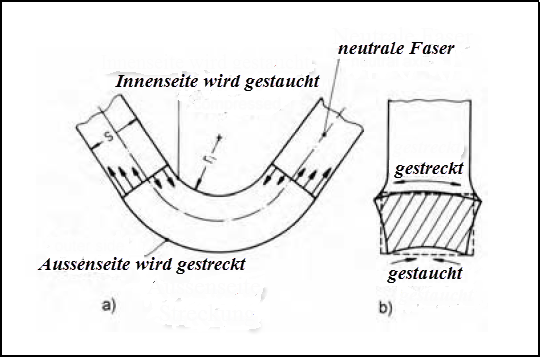
\includegraphics[scale=1]{neutralefaser}
\caption{Spannungen in der Deformierungszone beim Streckbiegen}
\label{fig:neutralefaser}
\end{figure}
In Hinblick auf die Serienfertigung sind die in den für den Fertigungsprozess  Streckbiegen durchzuführenden Versuchsserien, bei denen unter Verwendung von Strangpressprofilen der Verdeckkastendeckel des Audi A3 Cabriolet's gefertigt wird, spezifische Problembereiche besonders zu beachten.\\
Kritisch sind hier vor allen Dingen Biegeschwankungen und nicht kontinuierliche Materialeinschnürungen,  welche häufig an den Verengungen der Biegeradien auftreten. Die einflussreichsten mechanischen Eigenschaften des Werkstoffes sind bei diesem Verfahren die Härte sowie die Streckgrenze.

\subsection{Kröpfen \label{sec:kropf}}
Der eigenartig anmutende Ausdruck \emph{Kröpfen} bedeutet eigentlich nur \emph{krumm biegen}\footnote{Vgl.\url{
http://woerterbuchnetz.de/DWB/?sigle=DWB&mode=Gliederung&lemid=GK14769
}[27.10.2013].}
Bei dem Umformprozess Kröpfen werden von den  Enden der Zierleisten zu nächst die auf den Innenseiten verlaufenden Stege  abgefräst.  Daraufhin werden sie in der Kröpfeinheit (siehe \fref{fig:kropfeinheit}) auf dem Kröpfstein justiert und von einem Niederhalter durch die Anpresskraft einer Gasdruckfeder angepresst. Nun fährt, angetrieben durch einen Hydraulikzylinder, der Kröpf- oder auch Ziehstempel herunter und kantet das Material ab. Im Anschluss daran wird die Stirnseite der Kröpfung (siehe \fref{fig:kropfinstirn}) noch beschnitten.
\begin{figure}[!htb]
\centering
\hfill
\subfloat[Bezeichnungen \label{fig:kropfeinhzeich}]{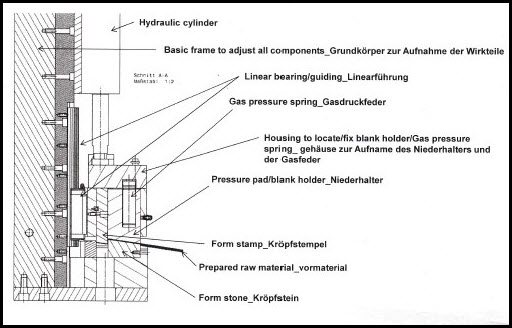
\includegraphics[scale=.715]{kropfeinhzeich}}
\hfill
\subfloat[Kröpfstein\label{fig:einheit}]{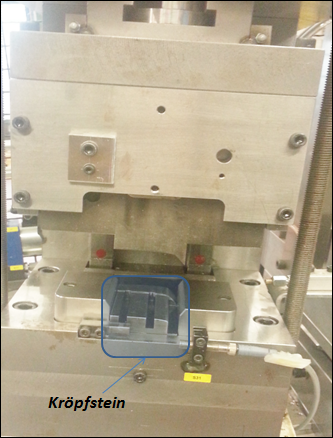
\includegraphics[scale=.5]{kropfeinheit}}
\hfill
\caption{Kröpfeinheit }
\label{fig:kropfeinheit}
\end{figure}

\begin{figure}[!htb]
\centering
\hfill
\subfloat[Kröpfung mit Fräsbereich  \label{fig:kropffrasbereich}]{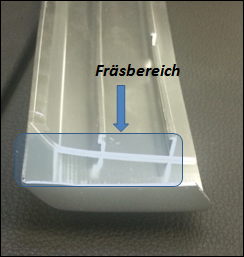
\includegraphics[scale=.822]{kropffrasbereich}}
\hfill
\subfloat[Kröpfung \label{fig:kropfung}]{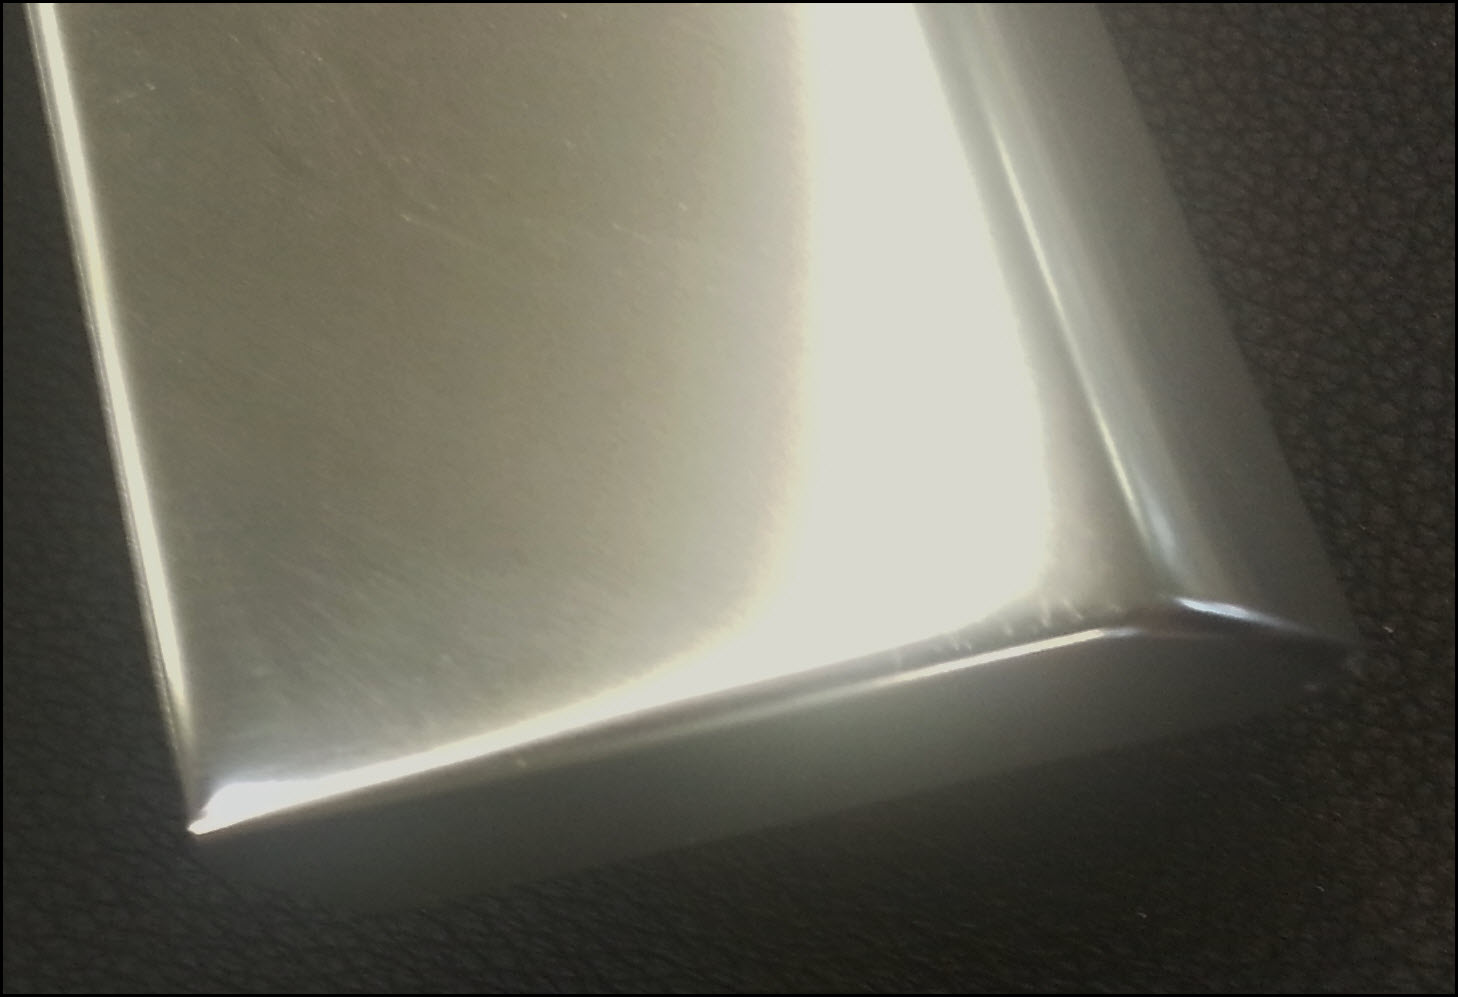
\includegraphics[scale=.16]{kropfung}}
\hfill
\caption{Kröpfung innen und Stirnseite }
\label{fig:kropfinstirn}
\end{figure}


 
Problembereiche sind hier zu erst einmal die Fräsprozesse. Schon bei geringsten Unterschieden in der Materialabnahme sind Fehlstellen in der Oberflächenqualität der Radien bei einer Sichtprüfung zu erkennen. Auch der Ziehstempel und der Kröpfstein lassen Spuren auf der Oberfläche zurück. Ein nicht zu vernachlässigender Aspekt sind auch Verschleiß des Werkzeugmaterials bei diesem Verfahren. So kommt es gerade bei Ziehstempeln aus Stahl oft zu Kaltaufschweißungen. Hier liegt nahe auch andere Werkzeugmaterialien in Versuchsreihen zu erproben.
\medskip

Hervorzuheben sind folgende, aus dem Kröpfprozess resultierende, Qualitätsbeeinträchtigungen:
\begin{itemize}
\item Orangenhaut (siehe \fref{sec:orangenhaut})
\item Materialungänzen bedingt durch Materialschwankungen
\item Abweichungen des auf das Kröpfen angepassten Fräsbildes
\end{itemize}











\subsection{Methode Messauswertung}
Es wurde bei der Auswertung von Messreihen in dieser Untersuchung vorwiegend die \textbf{\emph{empirische}} Standardabweichung 
\begin{equation}s= \sqrt{\frac{\sum \limits_{i=1}^n (x_i - \bar{x})^2}{n-1}}\end{equation}  verwendet, welche für solche Operationen von der Fachliteratur empfohlen wird.\footcite[Vgl.][301]{mf} Der Unterschied zur Standardabweichung \begin{equation} \sigma = \sqrt{\frac{\sum \limits_{i=1}^n (x_i - \bar{x})^2}{n}}\end{equation}  ist das \emph{Teilen} durch \textbf{n-1} anstatt durch lediglich \textbf{n}.
 An dieser Stelle eine kurze Beleuchtung des Sachverhaltes  (in Anbetracht der Erläuterungen von Dr. Guido Pinkernell\footnote{\url{www.ti-unterrichtsmaterialien.net/imgserv.php?id=pinkernell_106.pdf}[10.11.2013].‎}, welche exzellent  den Sachverhalt beleuchten)\footnote{Herv. d. Verf.}.



Die \textbf{\emph{empirische}} Standardabweichung berechnet das Streuungsmaß einer \emph{Stichprobe} im Gegensatz zur Standardabweichung die sich auf eine \emph{Grundgesamtheit} bezieht. Bei Stichproben wir die \emph{empirische} Standardabweichung vorgezogen da dort in der Regel die \emph{wirkliche Streuung} unterschätzt wird. Die \emph{empirische} Standardabweichung ist wegen des Teilers n-1 grundsätzlich etwas größer als die Standardabweichung, bei großem n liefern aber beide nahezu gleiche Ergebnisse, welches ja nur eine logische Konsequenz ist, denn je größer die Stichprobe desto näher kommt sie an die Grundgesamtheit.

\medskip

Durch das Quadrieren der einzelnen Abweichungen ($ x_i-\bar{x}$) und Addieren der einzelnen Abweichungsquadrate erhält man nur positive Beträge in denen eine Überbetonung einzelner Ausreißer erzielt wird.
Die empirische Standardabweichung ist   eines der wichtigsten Vergleichsparameter in der Statistik und bietet sich zur Analyse der Versuchsreihen besonders an, da sie von Extremwerten nicht stark beeinflusst wird.\footcite[Vgl.][54]{gst} Bei der Auswertung von Messbereichen, die für unsere Problemstellung besondere Signifikanz haben, wird zusätzlich der Fehler mit Hilfe der  \emph{Standardabweichung des Mittelwertes}  \begin{equation} \Delta\bar{x}= t_{0,95} \cdot \sqrt{\frac{\sum \limits_{i=1}^n (x_i - \bar{x})^2}{(n-1)\cdot n}}\end{equation}  angegeben.\footcite[Vgl.][16]{ph} Da bei den Versuchsserien eine nicht allzu große Stückzahl ($ n=16-20 $) bearbeitet wurde,  ist auch der für die international geforderte statistische Sicherheit zu berücksichtigende \emph{P} Wert mit dem $ t_{0,95} $ Faktor in die Berechnungen eingegangen.\footcite[Vgl.][609]{tp}  Es sei noch bemerkt, dass der Fehler nach DIN 1333 jeweils auf die erste signifikante Stelle gerundet wurde.\footcite[Vgl.][612]{tp}
 	 	
 	

 	
 	 	


\subsection{Chargenvergleich Streckbiegen}
Zur Versuchsdurchführung wurden drei Materialchargen zu jeweils 20 Profilen des Werkstoffes EN AW 6060 (Legierungsnummer EAL-6048 \emph{Alminox}, AlMgSi\,0,5) mit den Materialbezeichnungen F17 (T61/Charge 1) und Fxx (T4/Charge 2) sowie das ursprünglich zur Serienfertigung vorgesehene Material F13 (T4)  gegenübergestellt (eine Übersicht der relevantesten Eigenschaften ist in \fref{tab:chargeneigenschaften} aufgeführt).
\begin{table}[htbp]
\caption{Gegenüberstellung der mechanischen Eigenschaften (Laborwerte) der Chargen}
\label{tab:chargeneigenschaften}
\centering
\begin{tabular}{lllll}
\toprule
Material & Zugfestigkeit & Streckgrenze & Bruchdehnung & Zustand \\
Charge &  Rm [\si{\newton\per\milli\meter\squared}] &  $R_{p0,2}$ [\si{\newton\per\milli\meter\squared}] &  $A_{50}$ [\%] & \\
\midrule
1.F17 & 160,25 & 85,55 & $ 12,3 $ & T61 \\
2.Fxx & 152,4 & 74,65 &  $ 11,65 $ & T61 \\
3.F13 Serie & 149,3 & 70,55 & 20,41  & T4 \\
\bottomrule




\end{tabular}
\end{table}


 Die Chargen 1 und 2 wurden auch mit der herkömmlichen Zustandsbezeichnung T61 (lösungsgeglüht, nicht vollständig warmausgelagert, überaltert)\footnote{Vgl.\url{http://www.unibw.de/lrt5/lehre/praktikum/zusatzinformationen/download4/at_download/down1}[25.11.2013].} bezeichnet während das Serienmaterial im Zustand T4 (lösungsgeglüht, kaltausgelagert) bestellt wurde. \\
 Unter Überalterung versteht man  den Prozess der Vereinigung von  submikroskopischen Ausscheidungen die sich  in der Anzahl verringern jedoch als Ausscheidung größer werden und so eine Abnahme der Festigkeit herbeiführen.\footcite[Vgl.][52]{wki}\\
  Lösungsglühen erfolgt durch Glühen im Bereich der homogenen Mischkristalle welches das   Lösungsvermögen der Mischkristalle begünstigt, Ausscheidungen können so gelöst werden.\\
   Unter Auslagern versteht man Liegenlassen bei Raumtemperatur (Kaltauslagern) oder bei  höheren Temperaturen (Warmauslagern), meistens zwischen 100 und 220 Grad Celsius, über einen bestimmten Zeitraum um so die Eigenschaften des Werkstoffes zu beeinflussen.\footcite[Vgl.][213]{wk}
Ein typischer Aushärtungsprozess läuft nach folgendem Schema ab:

\begin{enumerate}
 \item Lösungsglühen aller Ausscheidungen in einem homogenen Mischkristall 
 \item Abschrecken
 \item Auslagern 
 \end{enumerate}
 
   
 
 

Die Zusstandsbezeichnungen F17, F13 und Fxx beziehen sich nach DIN 755-2 auf die Zugfestigkeit. Fxx ist allerdings eine firmeninterne Bezeichnung und bedeutet das ein  vorgezogener Kaltauslagerungsprozess durchgeführt wurde um das Strangpressprofil zu "`\emph{stabilisieren}"'. Das bedeutet ein gewisses "`Einfrieren"' des Gefüges in den momentanen Zustand um Veränderungen desselbigens auch bei nicht vorgesehener längerer Lagerung zu verhindern. Nach Auskunft des Lieferanten ist Fxx leicht wärmebehandelt worden.


 Bei Charge 2 (Fxx) schieden zwei Profile aufgrund von Biegefehlern aus. Die Proben wurden streckgebogen und auf einer Messlehre  mit 40 Messpunkten (Messpunkte MP1a bis MP10d) vermessen. Die Messbereiche, Messpunkte und Messuhren wurden, zur besseren Übersicht, mit Farben markiert (siehe \fref{fig:messpunktevdkda3}).  \\
 And den Messpunkten wurden folgende Messbereiche ermittelt:
 \begin{description}
 \item[MP1a-MP10a] Kontur aussen (grün)
 \item[MP1b-MP10b] Spalt (gelb)
 \item[MP1c-MP10c] Wölbung oben innen (rot)
 \item[MP1d-MP10d] Wölbung oben aussen (blau)
 \end{description}
\begin{figure}[!htb]
\centering
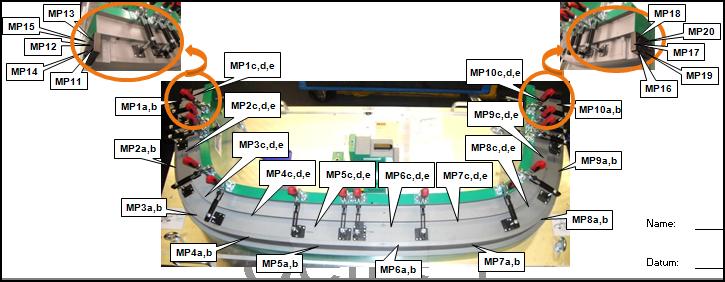
\includegraphics[width=1\linewidth,height=.2\textheight]{messpunktevdkda3}
\caption{Messpunkte Biegelehre}
\label{fig:messpunktevdkda3}
\end{figure} 
 
 
 
 
Das Messen erfolgte durch Abfahren aller Messpunkte mit den zu den spezifischen Messbereichen zu verwendenden Messuhren (siehe \fref{fig:messverfahren}). Ein negativer Messwert lässt auf eine Verkleinerung des Messbereiches schließen. Eine Ausnahme hierzu ist der Messbereich "`\emph{Spalt vorne unten}"' welcher  bei negativen Werten eine Vergrößerung bedeutet.\\
 Alle relevanten Messergebnisse (mit Ausnahme der Messpunkte MP1b und MP10b bei Charge 1, welche nicht zu ermitteln waren) wurden in Tabellen eingetragen und  der Mittelwert sowie die Standardabweichung
 ermittelt. Darüber hinaus erfolgte eine Gegenüberstellung der spezifischen Werte.\\
Da aufgrund der vielen Messpunkte  sehr umfangreiche Auswertungen durchgeführt wurden,  sind hier die für die Problematik Ausschlaggebendsten näher betrachtet worden. Alle weiteren Messergebnisse und Visualisierungen sowie Dokumentationen sind dem Anhang zugefügt. 
\begin{figure}[!htb]
\centering
\hfill
\subfloat[Messlehre  \label{fig:messlehre}]{\includegraphics[scale=.0877]{Messlehre}}
\hfill
\subfloat[Messung "`Kontur aussen"' \label{fig:messvdkd}]{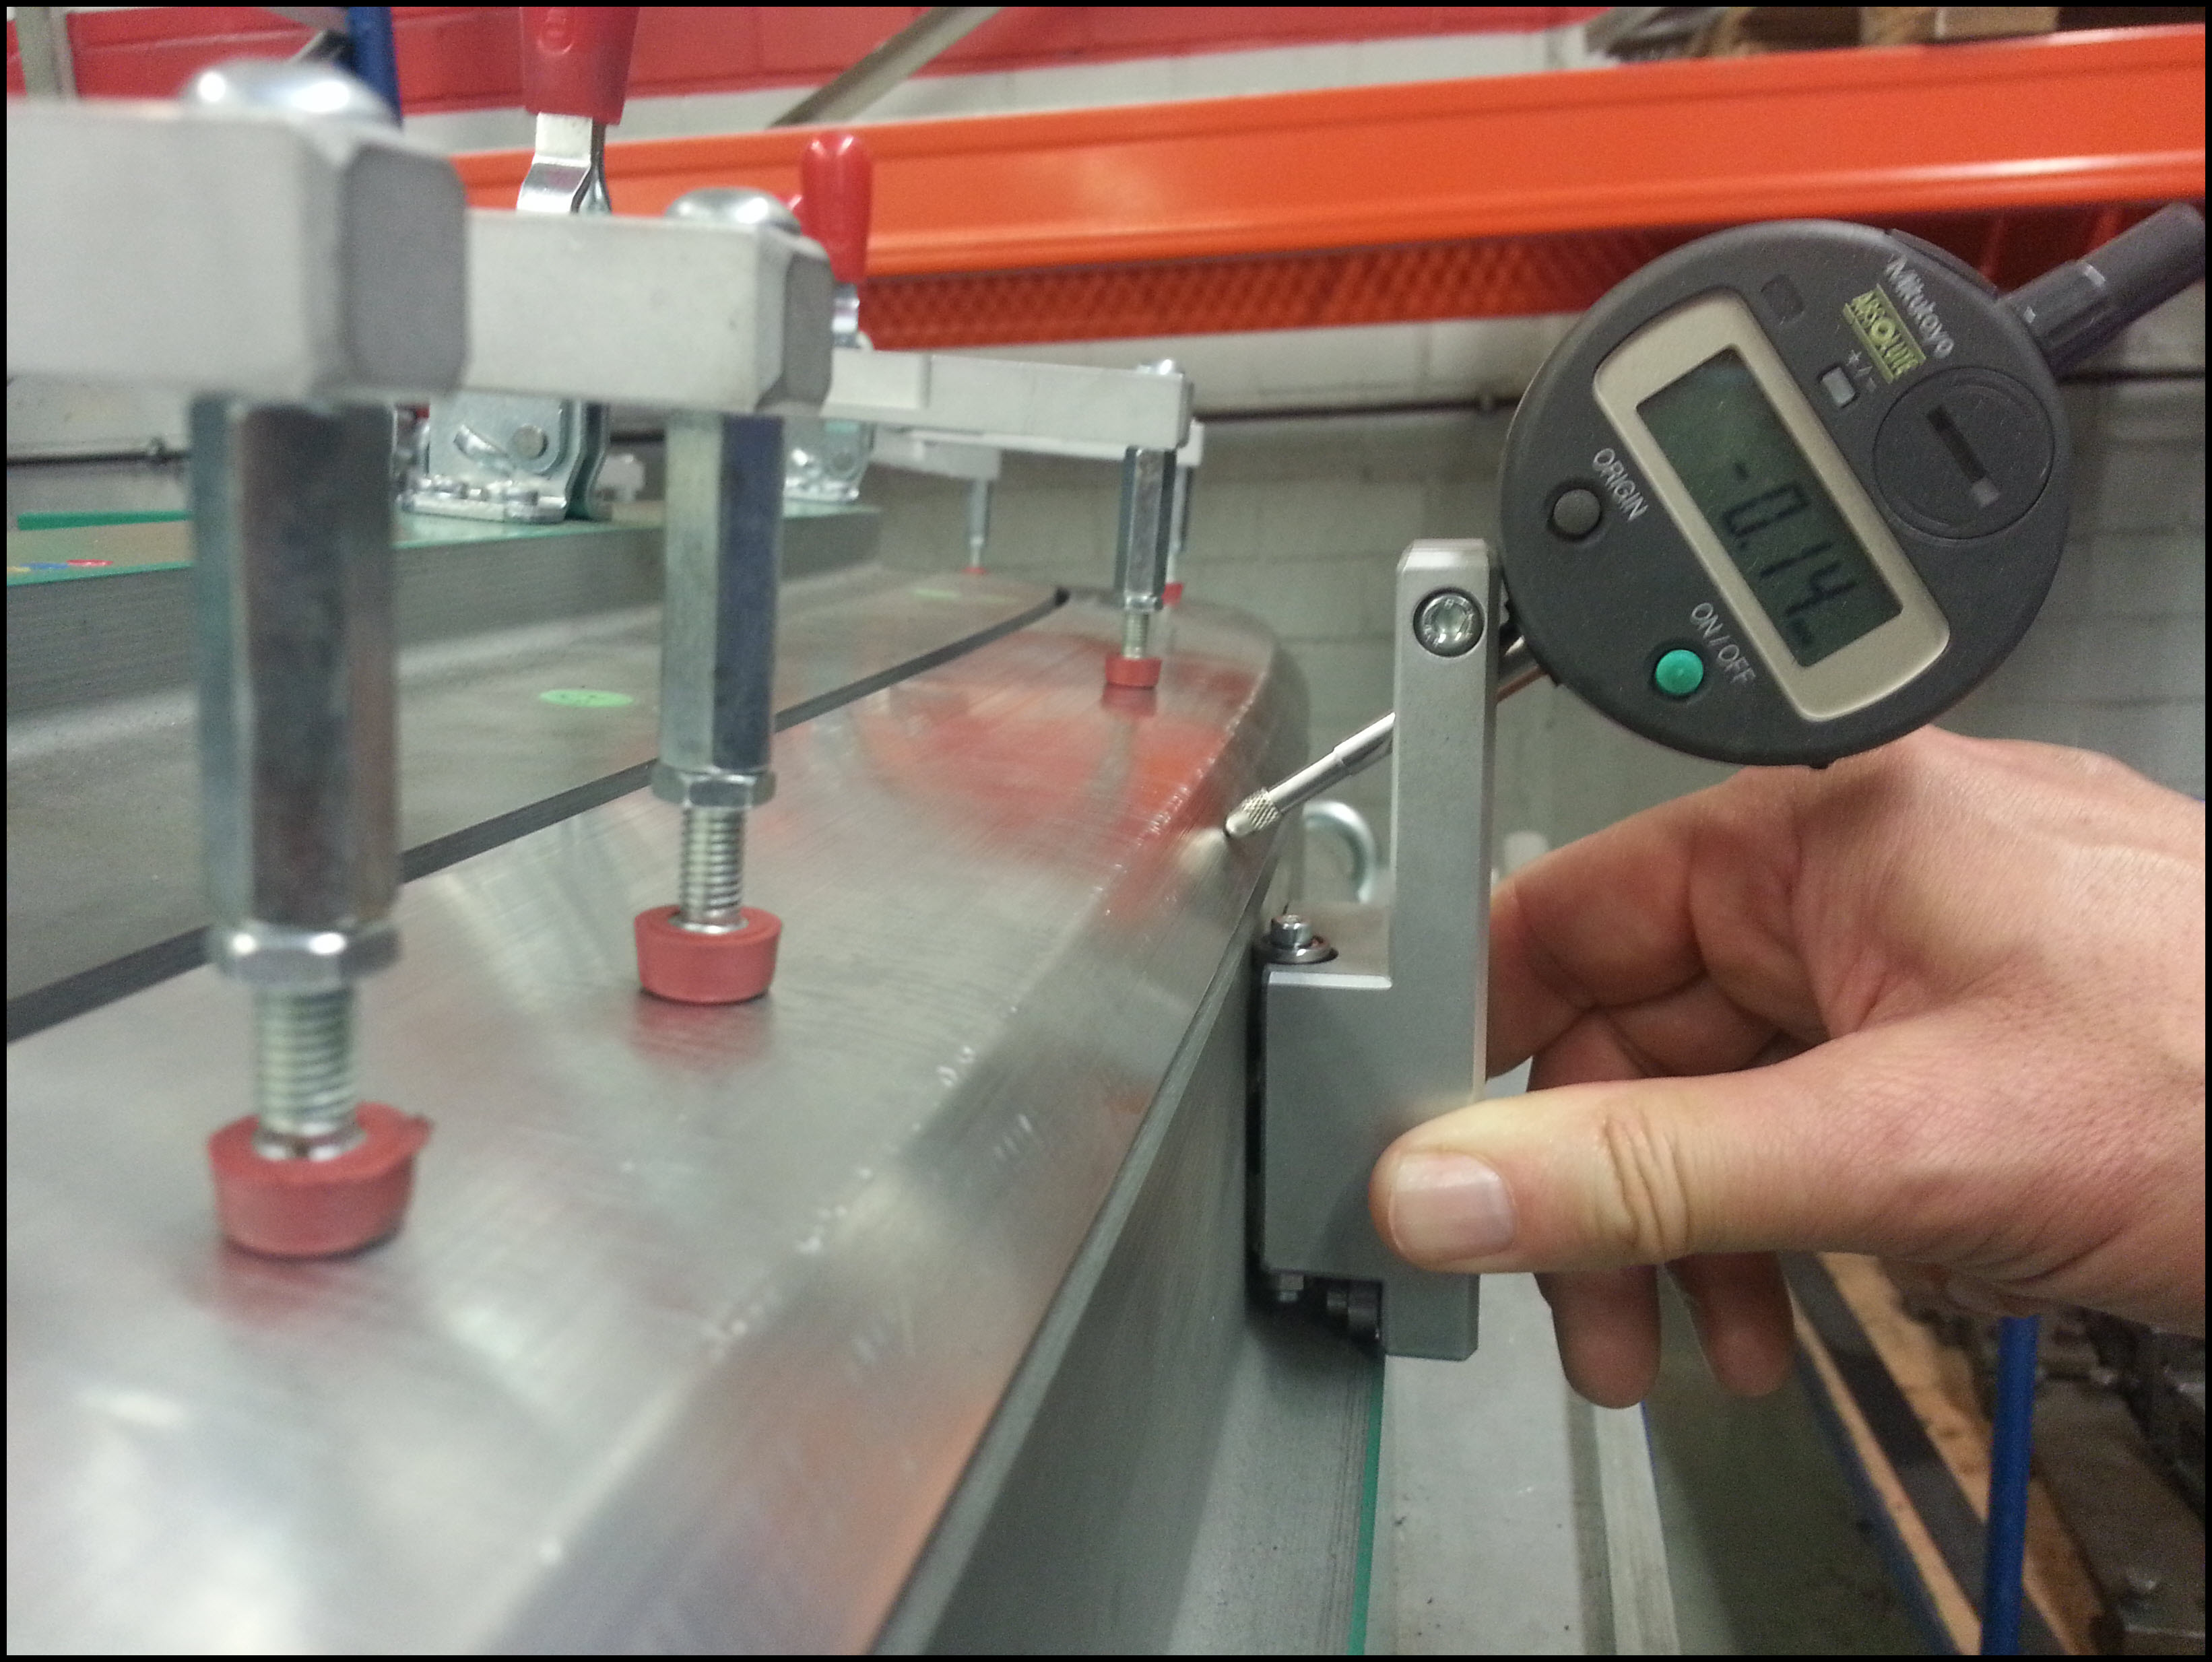
\includegraphics[scale=.042]{messvdkd}}
\hfill
\caption{Messverfahren an der "`Biegelehre"' }
\label{fig:messverfahren}
\end{figure}


Der für das Streckbiegen aussagekräftigste Parameter ist der Messbereich "`\emph{Kontur aussen}"' da er dem Verlauf der Biegelinie entspricht. Besonders an den Messpunkten MP1a und MP10a sind die Auswirkungen der Rückfederung zu beobachten. Ein Vergleich der Chargen ist in \fref{tab:mwertstandstreck} übersichtlich dargestellt. Ein visueller Vergleich der Standardabweichungen der "`Kontur aussen"' ist in \fref{fig:svstb} aufgeführt.
\begin{figure}[!htb]
\centering
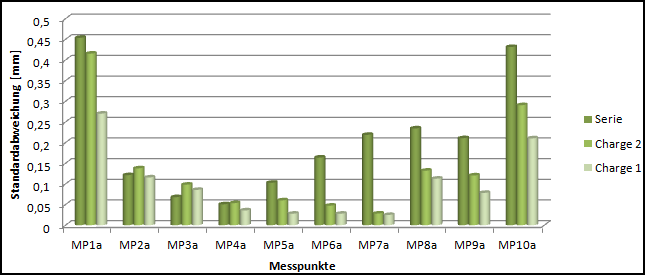
\includegraphics[width=1\linewidth,height=.3\textheight]{standardstreckb}
\caption{Überlagerung Standardabweichungen "`Kontur aussen"' Streckbiegen}
\label{fig:svstb}
\end{figure}
Dort ist zu sehen, dass das Material F17 (Charge 1) an fast allen Messpunkten die geringste Standardabweichung aufweist. Lediglich bei Messpunkt MP3a liegt sie in nicht großem Abstand zwischen dem Fxx (Charge 2) und dem F13 (Serie) Material.

Ein Vergleich der Mittelwerte (Kontur aussen) der Chargen (siehe  \fref{fig:mitstrckb}) ergibt, dass and den Messpunkten MP1a, MP2a, MP9a und MP10a  Charge 1 (F17) die größte Rückfederung nach dem Streckbiegeprozess auftritt.






\begin{table}[htbp]
\caption{Messwerte und Standardabweichungen Streckbiegen "`Kontur aussen"'} 
\label{tab:mwertstandstreck}
\vskip\abovecaptionskip



\footnotesize
   \begin{tabular}{cccccc}
   \toprule
   & \multicolumn{5}{c}{Messwert $x =  (\bar{x} \pm \Delta x)  $[mm]}\\
   \cmidrule(ll){2-6}
   Material    & MP1a & MP2a & MP3a & MP4a & MP5a \\  
   
   \midrule
  
   F17& $ 1,95\pm 0,13 $ & $0,72 \pm 0,06 $ & $0,60 \pm 0,04 $ & $ 0,028 \pm 0,017 $ & $-0,297 \pm 0,014$ \\
    Fxx & $0,81 \pm 0,21 $ & $0,34 \pm 0,07 $ & $0,15 \pm 0,05 $ & $0,021 \pm0,027 $ & $ -0,188\pm0,030$ \\
   F13  Serie & $-0,66 \pm0,22 $ & $-0,13 \pm 0,06 $ & $-0,38 \pm 0,04$ & $ 0,028\pm0,024 $&$0,00 \pm0,05 $ \\
     \bottomrule
     \toprule
  Material   & MP6a & MP7a & MP8a & MP9a & MP10a  \\
  \midrule
      F17&   $-0,368 \pm0,014 $&$-0,293 \pm0,012 $&$ 0,46 \pm 0,06 $&$ 1,31\pm 0,04$&$2,96 \pm0,10 $ \\
Fxx &$-0,233 \pm0,024 $&$-0,251 \pm0,015 $&$-0,17 \pm0,07 $&$0,57 \pm0,06 $&$1,37 \pm0,15 $ \\
  F13 Serie & $-0,04 \pm0,08 $&$ -0,16\pm0,11 $&$-0,55 \pm0,11 $&$0,04 \pm  0,10$&$-0,08 \pm0,21$ \\
     
     \bottomrule
      
     &&&&&\\
     &&&&&\\
     &&&&&\\
     &&&&&\\
     &&&&&\\
     
     \toprule
      & \multicolumn{5}{c}{Standardabweichung s [mm]}\\
   \cmidrule(ll){2-6}
   Material    & MP1a & MP2a & MP3a & MP4a & MP5a \\ 
   \midrule
    F17&0,270&0,116&0,086&0,036&0,028\\
    Fxx &0,416&0,138&0,098&0,053&0,060\\
    F13 Serie&0,454&0,121&0,068&0,051&0,103\\
     \bottomrule
     \toprule
  Material    & MP6a & MP7a & MP8a & MP9a & MP10a  \\
  \midrule
    F17 &0,028&0,025&0,113&0,078&0,210\\
 Fxx   &0,048&0,028&0,132&0,121&0,291\\
F13 Serie &0,164&0,219&0,235&0,211&0,432\\ 
   \bottomrule 
         
   \end{tabular} 
\end{table}

\begin{figure}[!htb] 
\centering
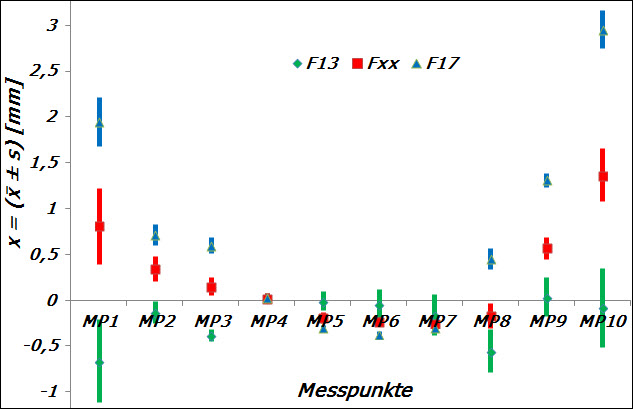
\includegraphics[width=1\linewidth,height=.3\textheight]{mitkontausstrckb}
\caption{Vergleich Mittelwerte "`Kontur aussen"' Streckbiegen}
\label{fig:mitstrckb}
\end{figure}

\newpage

\subsubsection{Ausblick}
In folge der Überlagerung der Standardabweichungen (Streckbiegen "`Kontur aussen"') der untersuchten Chargen unter dem Gesichtspunkt der Mindestzugfestigkeiten (siehe \fref{fig:standzugrel}) ist einzusehen, dass das Material F17 (Charge 1) bei einer Mindestzugfestigkeit von Rm = 160  \si{\newton\per\milli\meter\squared}  die geringste Standardabweichung hat. Bei Werten von s = (0,025  bis 0,270) \si{\milli\meter}  ist davon auszugehen das auch größere Stückzahlen mit relativ geringen Prozessschwankungen zu fertigen sind. Hier müssen jedoch eventuelle Montageprobleme des Verdeckkastendeckels aufgrund der höheren Rückfederungswerte von {$x_{\text{Rückfeder}}$ = (-0,368  bis 2,96) \si{\milli\meter} berücksichtigt werden. Eine Tatsache die bei einer Spannweite von 3,328 \si{\milli\meter} schon einen beachtlichen Spielraum beim Einbau und bei der Passform bedarf.  % montage wegen der Toleranzen fragen
Hier ist das Ausmaß von Wölbungen und Spannungen nach und während der Montage schon genau zu untersuchen.

\begin{figure}[!h]
\centering
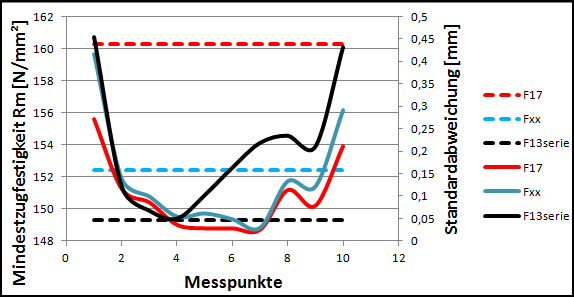
\includegraphics[width=1\linewidth,height=.3\textheight]{standzugrel}
\caption{Übersicht Mindestzugfestigkeit/Standardabweichung "`Kontur aussen"'}
\label{fig:standzugrel}
\end{figure} 

Zu einem ähnlichen Ergebnis kommen wir bei Betrachtung der Überlagerung der Chargen unter Berücksichtigung der Standardabweichung im Bezug zur Streckgrenze (siehe \fref{fig:standstreckrel}).
\begin{figure}[!h]
\centering
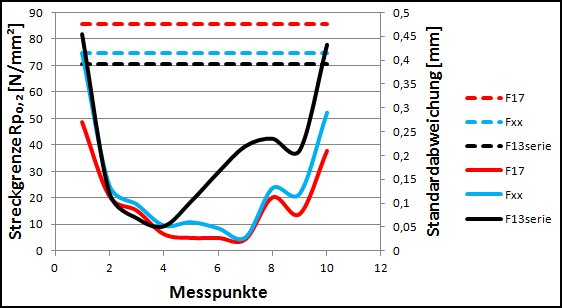
\includegraphics[width=1\linewidth,height=.3\textheight]{standstreckrel}
\caption{Übersicht Streckgrenze/Standardabweichung "`Kontur aussen"'}
\label{fig:standstreckrel}
\end{figure} 
Unter der Voraussetzung geringer Prozessschwankungen im Streckbiegeverfahren welche bei geringer Standardabweichung unter sorgfältiger und präziser Auswahl des Vormaterials durchaus zu realisieren sind, können die Ausschussrate sowie Kosten und Zeitverluste die durch ständiges Justieren der Streckbiegemaschine durch geschultes Personal entstehen, erheblich reduziert werden.

In Anbetracht der vorangegangenen Auswertung wurden noch einmal zwei Chargen (F19 und F18) bei dem Zulieferer, zu Versuchszwecken, bestellt. Möglicherweise ist hier ein Material herauszukristallisieren welches noch geringere Prozessschwankungen ermöglicht. Wir sind dabei von einer steigenden Zugfestigkeit ausgegangen da sich nach den Diagrammen in \fref{fig:standzugrel} und \fref{fig:standstreckrel} die Standardabweichung sowie Mindestzugfestigkeit und Streckgrenze gegenläufig verhalten.


 











\newpage
\section*{Anhang}


\printbibliography

\end{document}  
